\chapter{Расчет свободной энергии гидратации и адсорбции аминокислот} \label{part3_free_energy}


Данная глава иллюстрирует подходы молекулярного моделирования, позволяющие вычислять экспериментально измеримые термодинамические характеристики на основе молекулярно-динамических атомистических моделей.
В главе речь пойдёт об изучении гидратации боковых цепей аминокислот вблизи поверхности воды путём построения профилей свободной энергии на основании классических атомистических моделей молекул. Работа также имеет методологическое значение, поскольку в ней впервые предприняты попытки высокоточной численной оценки термодинамических параметров гидратации и адсорбции. Материалы данной главы следуют изложению приведенному в кандидатской депортации автора \cite{shaytan_thesis_kfmn_2010}, основаны на следующих статьях \cite{shaytan_free_2010,shaytan_solvent_2009} и материалах конференций \cite{shaytan_peptide_2006}. 

\graphicspath{{images/p3/}}

\section{Введение}
Применение молекулярной динамики к анализу поверхностных явлений нашло широкое применение за последние 20 лет поскольку позволяет дополнять экспериментальные данные и получать новой информацию на молекулярном уровне ~\cite{rev_benjamin_liq-liq_interf_1997,rev_pohorille_model_aq_sol_interf_2002}.
Величины, которые зачастую интересуют исследователя имеют статистическую природу (например, энергии связывания, коэффициенты распределения и т.д.), вычисление таких величин в компьютерном эксперименте требует серьёзной статистической выборки и значительных вычислительных ресурсов, одновременно накладывая ограничения на размеры и сложность молекулярных систем.

Методология вычисления свободных энегий (особенно с использованием стандартных силовых полей для белковых сруктур) получила много внимания за последнее десятилетие \cite{chipot_2002}, многие работы были посвящены систематической и критической оценке и сравнению методово, силовых полей, протоколов молекулярной динамики \cite{fee_maccalum_2003,fee_villa_2002,bar_comp,comp_fe_meth_2006,fee_hess_2006,fee_mobley_2007,shirts_waterff,shirts_proteinff,shirts_theory}. Однако эти работы в основном сводились к расчёту параметров в гомогенных системах (например, расчёту свободной энергии сольватации небольших молекул), в основном в воде, и в них не затрагивались вопросы расчёта систем с границей раздела фаз. Так было определено, что энергии гидратации боковых цепей аминокислот рассчитанные методом МД находятся в хорошей
 корреляции с экспериментальными данными, но систематически завышены. Разумным продолжением ряда этих работ является рассмотрение взаимодействия таких молекул не только с объёмом растворителя, но и с его границей. Если говорить о высокоточных оценках свободной энергии, то речь можно вести о достижении точности серьёзно выше $2 - 4$ кДж/моль, что является пределом точности, например, при предсказании связывания лигандов и белков при разработке лекарств. Если речь идёт не о качественных, а о количественных предсказаниях, то необходимая точность порядка 1 кДж/моль. Если же говорить, о настройке силовых полей на базе этих данных, то желаемая точность может быть около 0.1 кДж/моль.

\section{Постановка задачи}
Задачей данного исследования явился расчёт профилей свободной энергии для соединений аналогов нейтральных боковых цепей аминокислот на границе вода/пар с высокой точностью, вычисление энергий гидратации и адсорбции. В данной работе мы попытались обобщить и разработать наиболее точные и проверенные технологии таких расчётов, чтобы исключить зависимость результатов от методики расчётов. Для оценки качества результатов был проведён отдельный расчёт энергий гидратации молекул в объёме с использованием алгоритма Беннетта (Bennett acceptance ratio algorithm).
Для изучения были выбраны широко используемые модели соединений в силовом поле OPLS-AA \cite{opls-aa} с моделью воды  SPC.



\section{Teоретические аспекты расчета свободной энергии на границе фаз}
\subsection{Профиль плотности границы раздела вода-пар}

Профиль плотности границы раздела вода-пар удовлетворительно описывается полу-феноменологической капиллярно-волновой теорией (КВТ). Согласно КВТ \cite{cwt_stillinger_1965,rev_benjamin_liq-liq_interf_1997} профиль плотности может быть описан как некоторый молекулярный профиль, уширенный термическими капиллярными волнами. Экспериментальные результаты и результаты моделирования \cite{rev_surf_struct_penfold_2001,cap-simul_senapati_2001, int-wat-polar_rivera_2006} допускают, что толщина границы раздела зачастую может быть описана только капиллярными волнами, то есть является практически ступенчатой на молекулярном уровне. В этом случае профиль плотности может быть описан функцией интеграла ошибок:
\begin{equation}
\rho_z=\frac{1}{2}(\rho_L+\rho_V)-\frac{1}{2}(\rho_L-\rho_V)\mathrm{erfc}\left[\frac{(z-z_0)}{\sigma \sqrt{2}}\right]
\label{erf_prof}
\end{equation}
где $\rho_L$ и $\rho_V$ плотность жидкости и пара, а $\sigma$ толщина границы раздела.

Известной проблемой при моделировании границ раздела является зависимость толщины границы от линейных размеров поверхности $L_x$. Согласно КВТ имеется логарифмическая зависимость толщины от линейного размера (из-за зависимости от размера количества возможный волновых мод):
\begin{equation}
\sigma^2=\frac{k_BT}{2\pi\gamma}\ln{\left(\frac{L_{||}}{B_0}\right)}
\label{cap_wave_dep}
\end{equation}
где $\gamma$ поверхностное натяжение, $B_0$ характерная длина коротковолновой обрезки спектра, обычно полагаемая равной размеру молекулы.

В термодинамическом пределе (без учёта гравитации) толщина границы плоского раздела фаз - расходится для жидкостей только с взаимодействиями ближнего порядка при рассмотрении в трёх и менее измерениях \cite{nointin3d_robert_1985}.

\subsection{\label{pmf_theor_backgr}Теория профилей свободной энергии}

На рис. \ref{system} представлена геометрия двухфазной системы с плоской границей раздела, которая перпендикулярна оси Z. В системе присутствует вода, пар и тестовая молекула S, для которой мы хотим посчитать её профиль свободной энергии вдоль оси Z.
Система находится при постоянной температуре и давлении (за счёт хорошей сжимаемости пара). Предположим, что система описывается в классическом приближении, тогда система из N частиц описывается своей функцией потенциальной энергии  ~\cite{landau_tm} $U(\vec{q})$, зависящей от 3N обобщённых координат  $\vec{q}$. Чтобы отслеживать положение тестовой молекулы введём функцию $d_{z}(\vec{q})$, которая является проекцией расстояния между центрами масс тестовой молекулы и водного слоя на ось Z.
Основные формулы статистической физики \cite{stat_mech_book_2000},  которые нам нужны, это соотношения связывающие распределение вероятности, профили свободной энергии и потенциал средней силы.
В нашем случае вероятность найти молекулу S на расстоянии $z$ от центра масс водного слоя есть:
\begin{equation}
P(z)=<\delta(d_{z}-z)>=\frac{\int{\delta(d_{z}-z)e^{-U/kT}d\vec{q}}}{\int{e^{-U/kT}d\vec{q}}}
\label{probab}
\end{equation}
где $<...>$ усреднение по каноническому ансамблю, $k$ постоянная Больцмана, $T$ -температура. 

Зная распределение, мы можем рассчитать профиль свободной энергии:

\begin{equation}
W(z)=-kT\ln{P(z)}+F_0
\label{fe_prof}
\end{equation}

- где $F_0$ произвольная константа. В эксперименте профиль вероятности будет соответствовать профилю концентрации, предполагая, конечно, что раствор является разбавленным, или идеальным. Кирквуд~\cite{kirkwood} ввёл понятие потенциала средней силы (ПСС) и показал, что профиль потенциала средней силы с точностью до константы равен профилю свободной энергии. В нашем случае средней силой является средняя сила взаимодействия тестовой молекулы и водного слоя при условии, что проекция расстояния между центрами масс на ось Z фиксирована. Средняя сила задаётся как:
\begin{equation}
\overline{F(z)}=\frac{
 \int{<\delta(d_{z}(\vec{q})-z)>\nabla_{d_z}U(\vec{q})e^{-U/kT}d\vec{q}}
}
{\int{e^{-U/kT}d\vec{q}}}
\label{mf}
\end{equation}
где $\nabla_{d_z}$ оператор градиента, связанный с расстоянием вдоль оси Z между центрами масс.
Можно показать, что профиль свободной энергии и потенциал средней силы -- это одно и то же:

\begin{equation}
\frac{\partial W(z)}{\partial z}=\overline{F(z)}
\end{equation}

\subsection{\label{hfe_theor_backgr}К вопросу вычисления энергий гидратации}

В случае попарно-аддитивных молекулярных взаимодействий функцию потенциальной энергии можно разбить таким образом, чтобы выделить взаимодействие между тестовой молекулой и растворителем:
\begin{equation}
U(\vec{q},\lambda)=U_{wat}(\vec{q}_{wat})+\lambda U_{int}(\vec{q}_{wat},\vec{q}_{S})+U_S(\vec{q}_{S})
\label{pot_ener}
\end{equation}
\\
где $U_{wat}$,$U_{S}$,$U_{int}$, потенциальные энергии молекул воды, молекулы растворённого вещества и энергия их взаимодействия, соответственно.
Обобщённые координаты разбиваются удобным образом так, что $\vec{q_{S}}$ -- это координаты, описывающие конфигурацию молекулы S (молекулы растворённого вещества) в ящике с водой, $\vec{q}_{wat}$ -- координаты всех молекул воды.
$\lambda$ -- это параметр сопряжения, вводимый для последующих выкладок. При $\lambda=1$ и $\lambda=0$ взаимодействия между молекулой S и водой включены и отключены полностью, соответственно. 

Энергия гидратации, как показано в приложении -- это свободная энергия (работа) включения взаимодействий между молекулой S и остальным раствором в NPT ансамбле \cite{shaytan_free_2010}. 
Энергия гидратации Гиббса $\Delta G_{hydr}$ может быть выражена:
\begin{equation}
\Delta G_{hydr}=-kT \ln \left( \frac{\Delta (P,T,\lambda=1)}{\Delta (P,T,\lambda=0)} \right)
\label{hydr_fe_sim}
\end{equation}

где  $\Delta (P,T,\lambda)$ -- изотермо-изобарическая функция распределения вида:
\begin{equation}
\Delta (P,T,\lambda) \propto \frac{1}{N!}\int\int\int dPd\vec{q}\exp\left(-\left[U(\vec{q},\lambda)+PV\right]/kT\right)
\label{hydr_fe_expr}
\end{equation}
и N - число молекул воды. Такая формулировка верна в термодинамическом пределе  ($N\rightarrow\infty$) пока у нас есть одна молекула S.
Можно показать, что химический потенциал растворённого вещества (молекулы S) в идеальном растворе выражается как:
\begin{equation}
\mu_S=-kT\ln(1/c)+\Delta G_{hydr}
\label{chem_pot}
\end{equation}
где $c$ - концентрация растворённого вещества.

Таким образом с экспериментальной точки зрения свободная энергия гидратации может быть получена путём измерения концентрации вещества S в воде $c_{wat}$ и паре $c_{gas}$:
\begin{equation}
\Delta G_{hydr}^{exp}=kT\ln\left(\frac{c_{gas}}{c_{wat}}\right)
\label{hydr_energy_exp}
\end{equation}


\subsection{\label{ads_fe_theory}Энергии адсорбции}
Параметры, описывающие поверхностную активность веществ, обычно описываются в терминах теории адсорбции Гиббса (хотя есть и другие: Ван-дер-Ваальса, Кана-Хилларда). В теории Гиббса \cite{gibbs_ads_theory} поверхность раздела считается отдельной двумерной фазой, расположенной на поверхности раздела Гиббса (ПРГ), и характеризуется двумерными величинами концентрации, называемыми, избытками Гиббса $\Gamma^i$). Согласно Гиббсу, объёмные фазы характеризуются своими объёмными концентрациями вплоть до границы раздела, а любой избыток или недостаток вещества в районе границы раздела описывается соответствующими двумерными избытками Гиббса.
Зная профиль концентрации $c^i(z)$, а также величины концентрации в объёме $c^i_1$, $c^i_2$, избыток Гиббса может быть рассчитан по формуле:
\begin{equation}
\Gamma^i=\int_{-\infty}^{z_0}(c^i(z)-c^i_1)dz+\int_{z_0}^{\infty}(c^i(z)-c^i_2)dz
\label{excess}
\end{equation}
где $z_0$ - координата ПРД. Позиция ПРД обычно выбирается так, чтобы избыток Гиббса для растворителя был равен нулю.
В этих переменных можно записать уравнение адсорбции Гиббса, которое соотносит избыток Гиббса ($\Gamma^S$), концентрацию вещества в объёмной фазе ($c^S$) и поверхностное натяжение ($\gamma$):

\begin{equation}
\Gamma^S=-\frac{1}{kT}\frac{d\gamma}{d\ln{c^S}}
\label{GAE}
\end{equation}
Мерой поверхностной активности обчно считается отношение $\Gamma^S/c^S$ в пределе бесконечно разбавленного раствора ($c^S\rightarrow 0$).
Это отношение можно оценить путём измерения поверхностного натяжения при различных концентрациях, что следует из (\ref{GAE}):
\begin{equation}
\left. \frac{\Gamma^S}{c^S}  \right|_{c^S\rightarrow 0}=-\frac{1}{kT}\left. \frac{d\gamma}{dc^S} \right|_{c^S\rightarrow 0}
\label{exp_GE_conc_ratio}
\end{equation}
Понятие энергии адсорбции может быть далее введено, хотя оно остаётся до некоторой степени произвольно определённым, поскольку оно зависит от выбора стандартных состояний или толщины границы раздела (толщины поверхностного монослоя). Один из возможных вариантов состоит в определении величины толщины поверхностного слоя $\tau$, тогда энергию адсорбции можно записать в виде:
\begin{equation}
G_{ads}=-kT\ln{\frac{\Gamma^S}{c^S\tau}}
\label{ads_fe_eq}
\end{equation}
Однако при сравнении экспериментальных значений энергии всегда нужно обращать внимание на то, какому определению следовали экспериментаторы.




\section{Методы расчёта}
Для расчёта профилей использовался классический метод молекулярной динамики в комбинации с методом удерживающей силы для расчёта профилей свободной энергии. Для расчёта энергий гидратации в объёме использовался метод Беннетта. В данном разделе описывается модель силового поля, протоколы МД, а также методика расчёта. Более подробное описание нюансов протоколов и обоснование их выбора приведено в статье \cite{shaytan_free_2010}.

\subsection{\label{sec:forcefield}Силовое поле и модель}
Для создания модели было выбрано полноатомное силовое поле  OPLS-AA \cite{opls-aa}
и твёрдая (с фиксированными внутренними степенями свободы) модель воды SPC \cite{spc}. Основные характеристики модели воды представлены в таблице \ref{wat_param}. 
Атомы представляются как классические частицы, соединённые связями. Невалентные взаимодействия представлены потенциалами Леннард-Джонса и Кулона:
\begin{equation}
U^{nb}=\sum_{i<j}4\epsilon_{ij}\left[\left(\frac{\sigma_{ij}}{r_{ij}}\right)^{12}-\left(\frac{\sigma_{ij}}{r_{ij}}\right)^{6}\right]+\sum_{i<j}\frac{q_iq_j}{4\pi r_{ij}^2}
\label{non-bond}
\end{equation}
\begin{table}[p]

	\begin{tabular}{ccccccc}
$\sigma$, \AA & $\epsilon$, кДж/моль & $q_o$, $e$ & $q_h$, $e$ & $l_{OH}$, \AA & $\theta^{\circ}$ & P, D  \\
	\hline
3.166 & 0.65 & -0.82 & 0.41 & 1.0 & 109.47 & 2.27
\end{tabular}

	\caption{Основные характеристики модели воды SPC, включая параметры Леннард-Джонса $\sigma,\epsilon$, частичные заряды на кислороде ($q_o$) и водороде ($q_h$), длины связей, HOH угол ($\theta^{\circ}$) и дипольный момент ($P$).}
	\label{wat_param}
\vspace{2 in}
\end{table}
 

Валентные взаимодействия включали угловые, торсионные и ложно торсионные члены. 
Параметры потенциала Леннард-Джонса и заряды для соединений были взяты из работы \cite{shirts_proteinff}.
В таблице \ref{molecules} представлены 13 нейтральных аминокислот и соответствующие им соединения аналоги боковых цепей, которые изучались в данной работе.
\begin{table*}[p]

	\begin{tabularx}{\textwidth}{XXXX}
Аминокислота & Вещество аналог боковой цепи & Химическая формула & Сокр. обозначение \\
	\hline

аланин       & метан   					  & CH$_4$      						 &  ALA'  \\
валин     & пропан					    & C$_3$H$_8$ 							 &  VAL'  \\
лейцин & изобутан 					  & C$_4$H$_{10}$			 			 &  LEU'  \\
изолейцин    & н-бутан     					& C$_4$H$_{10}$						 &  ILE'  \\
цистеин   & метанэтиол 					& CH$_3$SH    						 &  CYS'  \\
метионин    & метилэтилсульфид  & C$_2$H$_5$SCH$_3$  			 &  MET'  \\
серин       & метанол				& CH$_3$OH        			   &  SER'  \\
треонин     & этанол								& C$_2$H$_5$OH      			 &  THR'  \\
тирозин& п-крезол						& C$_3$C$_6$H$_4$OH		 	   &  TYR'  \\
фенилаланин & толуол								& C$_6$H$_5$CH$_3$   			 &  PHE'  \\
триптофан    & 3-метилиндол 				& C$_6$H$_4$C$_2$HNHCH$_3$ &  TRP'  \\
аспарагин    & ацетамид					& CH$_3$CONH$_2$					 &  ASN'  \\
глутамин     & пропионамид					& C$_2$H$_5$CONH$_2$       &  GLN'  \\
\end{tabularx}
	
	\caption{Список 13 изученных нейтральных веществ - аналогов боковых цепей аминокислот, из названия, химические формулы и обозначения.}
	\label{molecules}

\end{table*}


\subsection{\label{sec:fep_method} Расчёт профилей свободной энергии}
Для расчёта профиля свободной энергии соединений на границе раздела фаз вода/пар была сконструирована модель границы раздела, см. Рис. \ref{system}. Прямоугольный слой воды толщиной 4 нм помещён в расчётную ячейку (3x3x20нм$^3$), чьи размеры постоянны в ходе моделирования. Количество молекул воды - 1173. Расчёты проводились в пакете GROMACS  v. 3.3.1 \cite{gromacs}. Для расчёта профиля свободной энергии использовался метод сдерживающей силы. С помощью алгоритма поддерживалась фиксированная проекция  расстояния между центрами масс молекулы и водного слоя на ось, перпендикулярную к поверхности. На каждом шаге измерялась сдерживающая сила, которую необходимо было прикладывать, чтобы это расстояние оставалось фиксированным. Для этого использовался, так называемый, GROMACS pull code, который поддерживал проекцию расстояния постоянной с использованием алгоритма SHAKE \cite{shake}. Исследуемая молекула помещалась на различных расстояниях от центра масс водного слоя, и для каждой такой системы после уравновешивания проводился расчёт длиной в 4 нс. Для каждой молекулы было рассчитано 80 точек: положение от -4 нм до 4 нм с шагом 0.1 нм. Мгновенная сила записывалась на каждом шаге, затем усреднялась. Профиль средней силы затем аппроксимировался кубическим сплайном, учитывая симметрию профиля относительно z=0 (см. Рис. \ref{4pmf}). Интегрированием профиля средней силы вычислялся профиль свободной энергии. Соответствующие теоретические формулы приведены в статье \cite{shaytan_free_2010}.

     
\begin{figure}
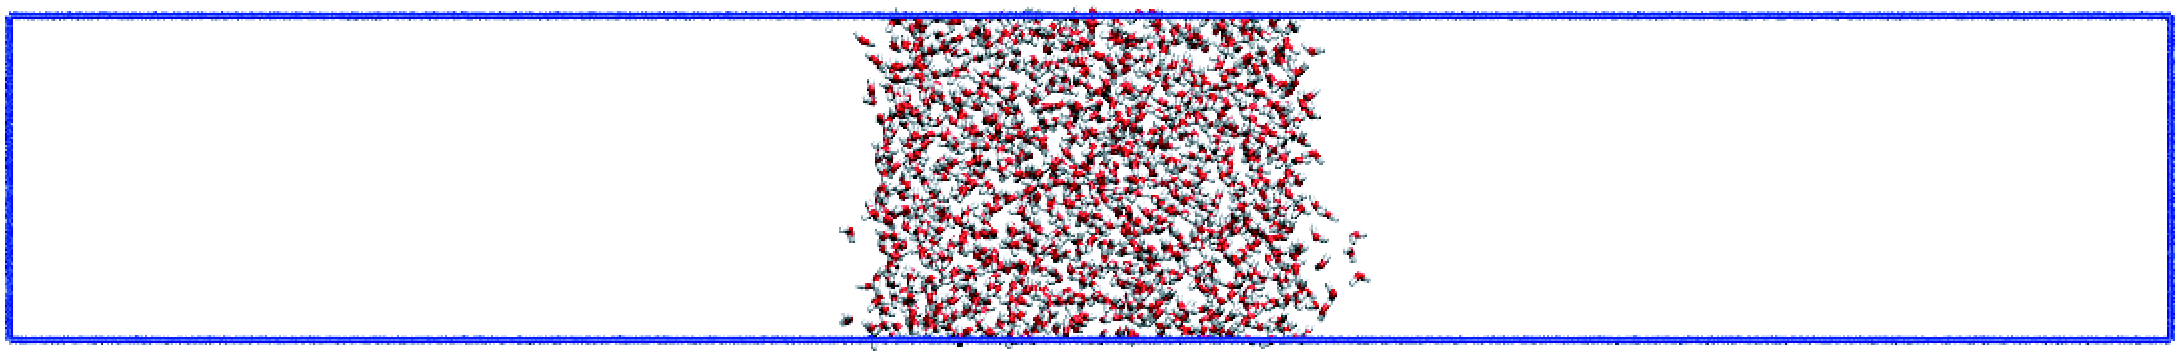
\includegraphics[width=17cm,height=2.5cm]{system}
\caption{\label{system} Мгновенное изображение модели системы с границей раздела вода/пар в периодической ячейке. Наиболее длинная сторона ячейки совпадает с нормалью к границе раздела (ось Z).}
\end{figure}


\subsection{\label{sec:hfe_method} Расчёт энергий гидратации}
Энергии гидратации рассчитывались по методу Беннетта \cite{bar} путём постепенного ``отключения'' взаимодействий между молекулой растворённого вещества и растворителем в ячейке, содержащей около 900 молекул воды.
Теоретические основы и детали метода Беннетта для оценок энергии гидратации могут быть найдены в работах других исследователей \cite{smith_bar,bar_comp,shirts_waterff}. Основные статистические соотношения приведены в статье \cite{shaytan_free_2010}.

Здесь мы приведём основные параметры нашего расчёта. Использовался стандартный термодинамический цикл: сначала молекула постепенно ``отключалась'' от среды путём зануления зарядов и параметров потенциала Леннард-Джонса, а затем проводился аналогичный коррекционный расчёт в вакууме, чтобы измерить поправку на внутримолекулярные взаимодействия. Отключение (мутация) молекулы в обоих случаях проводилась в 10 шагов. Сначала занулялись заряды, а потом отключались взаимодействия Леннар-Джонса. Электростатика отключалась в 2 шага, сначала заряды уменьшались в $\sqrt{2}$ раз, а затем занулялись. Взаимодействия Леннард-Джонса отключались в 8 шагов согласно формуле:
\begin{eqnarray}
U^{LJ}_{S}=\sum_{j}\sum_{i}f(i,j)\lambda4\epsilon_{ij}& & \nonumber \\
  \times\left(\frac{\sigma_{ij}^{12}} {(\alpha\sigma_{SC}^6(1-\lambda)+r_{ij}^6)^2}-\frac{\sigma_{ij}^6}{\alpha\sigma_{SC}^6(1-\lambda)+r_{ij}^6}\right) & &
\end{eqnarray} где $i$ поробегает по всем атомам растворённого вещества, $j$ по всем атомам в системе, $f(i,j)$ - ответственна за исключение взаимодействия между атомами связанными валентно. $\alpha=0.5,\sigma_{SC}=0.3\;нм$. В такой форме этапы мутации соответствовали параметрам $\lambda=1,0.8,0.7,0.6,0.5,0.4,0.3,0.2,0$. Для каждой стадии осуществлялись расчёты длиной 5 нс. Конфигурации записывались каждые 2 пс. Эти конфигурации обрабатывались по алгоритму Беннетта, чтобы получить оценку разницы свободной энергии между смежными состояниями.

\subsection{\label{sec:simprot}МД протокол}
В качестве алгоритма для получения выборок мы использовали динамику Ланжевена, согласно уравнению: 
\begin{equation}
m_i\frac{d^2\mathbf{r}_i}{dt^2}=-m_i\xi_i\frac{d\mathbf{r}_i}{dt}+\mathbf{F}_i(\mathbf{r}_i)+\hat{\mathbf{r}}_i
\label{langevin}
\end{equation}
где $\xi_i$ константа трения, а $\hat{\mathbf{r}}_i(t)$ шумовой процесс $<\hat{\mathbf{r}}_i(t)\hat{\mathbf{r}}_j(t+s)>=2m_i\xi_ikT\delta(s)\delta_{ij}$. Ланжевенова динамика является точным методом, позволяющим реализовать изотермический ансамбль.

Использовался пакет GROMACS  v 3.3.1 \cite{gromacs}, скомпилированный с двойной точностью. Уравнения Ланжевена интегрировались с исользованием лип-фрог алгоритма третьего порядка \cite{leap_frog_lang_gunsteren_1988} с шагом 2 фс. Для фиксации длин связей использовались алгоритмы  LINCS \cite{lincs} и SETTLE \cite{settle}. Расчёты проводились при постоянной температуре 300 К.
Константа трения $\xi$ для каждого атома рассчитывалась как $\xi_i=m_i/\tau_T$, где $\tau_T=1$ пс, $m_i$ -- масса атома. Для расчётов энергии гидратации использовался алгоритм задания изобарического ансамбля Паринелло-Рамана \cite{barostat} при 1 атм, время релаксации 2 пс, сжимаемость $4.5*10^{-5}$ бар$^{-1}$.  
Для расчёта электростатических взаимодействий использовался метод PME \cite{pme,pme2} с радиусом обрезки в прямом пространстве 1.3 нм и PME-порядком 6. Максимальное расстояние в пространстве фурье (maximum Fourier spacing) задовалось равным 0.12 нм.
Относительная толерантность между вкладами в энергию прямого и обратного пространств $10^{-5}$. Для потенциала Леннард-Джонса использовалась свитч функция, сглаживающая потенциал между 1.0 и 1.2 нм. Коррекционая поправка  (long-range correction) учитывалась при вычислении энергии и давления.

\section{Результаты и обсуждение}

\subsection{\label{sec:wat_res}Свойства водного слоя}
Чтобы оценить правильность нашей модели, рассмотрим сначала свойства модели границы раздела фаз. Расчёт длиной в 50 нс был проведён для того, чтобы оценить профиль плотности, поверхностный потенциал и ориентационное поведение молекул воды.
Профиль плотности идеально описывается уравнением \ref{erf_prof} с параметрами $ \sigma=0.14 $ нм,
 $ \rho_g=0.2 $ kg/m$^3$ и $ \rho_L=970.5 $ kg/m$^3$, поверхность раздела Гиббса находится в точках $z=\pm2.007$ нм. Толщина границы, рассчитанная из теории капиллярных волн  $\sigma_{CWT}=1.45$ \AA, хорошо согласуется с данными моделирования ($ \sigma=0.14 $ нм).

% \begin{equation}
% \rho_z=\frac{1}{2}(\rho_L+\rho_V)-\frac{1}{2}(\rho_L-\rho_V)\mathrm{erfc}\left[\frac{(z-z_0)}{\sigma \sqrt{2}}\right]
% \label{erf_prof}
% \end{equation}


\begin{figure}
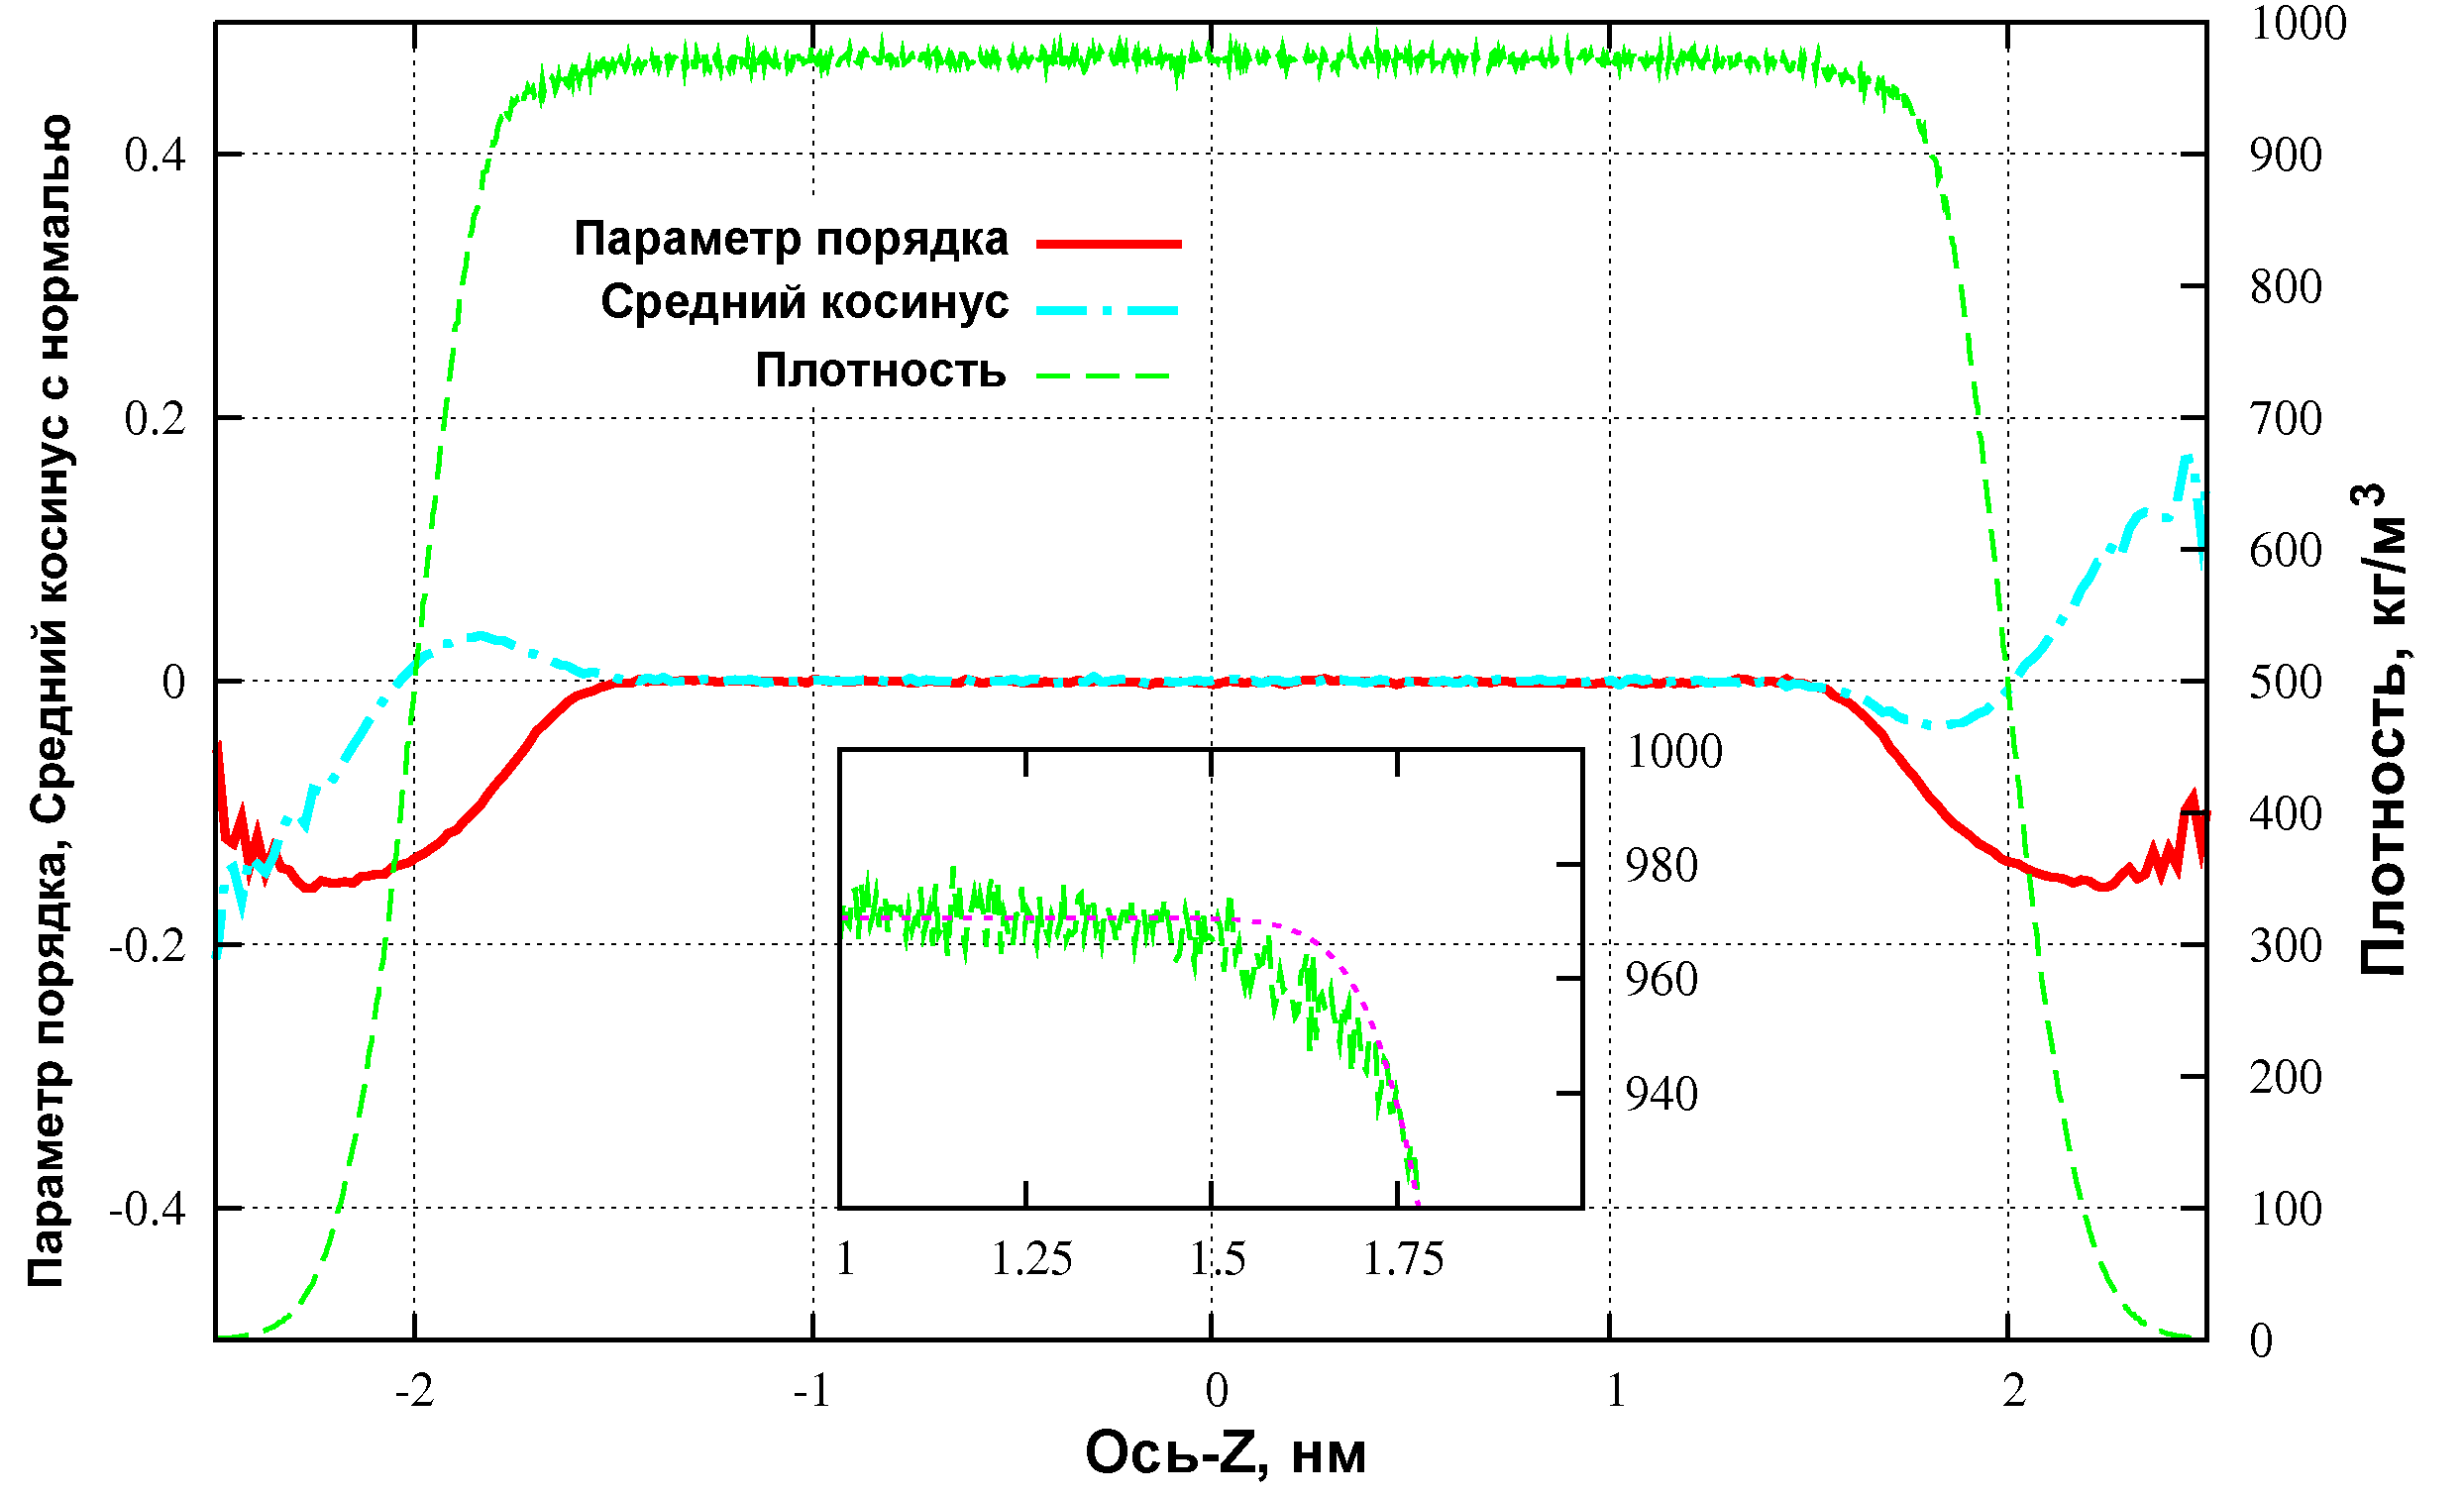
\includegraphics[width=16cm,height=10cm]{orddens}
\caption{\label{orddens} Профиль плотности водного слоя (пунктирная линия) и средние ориентационные характеристики дипольного момента молекул воды: средний косинус угла с нормалью (пунктирно-точечная линия),  параметр порядка $P_2(\cos(\theta))$ (сплошная линия). }
\end{figure}

\begin{figure}
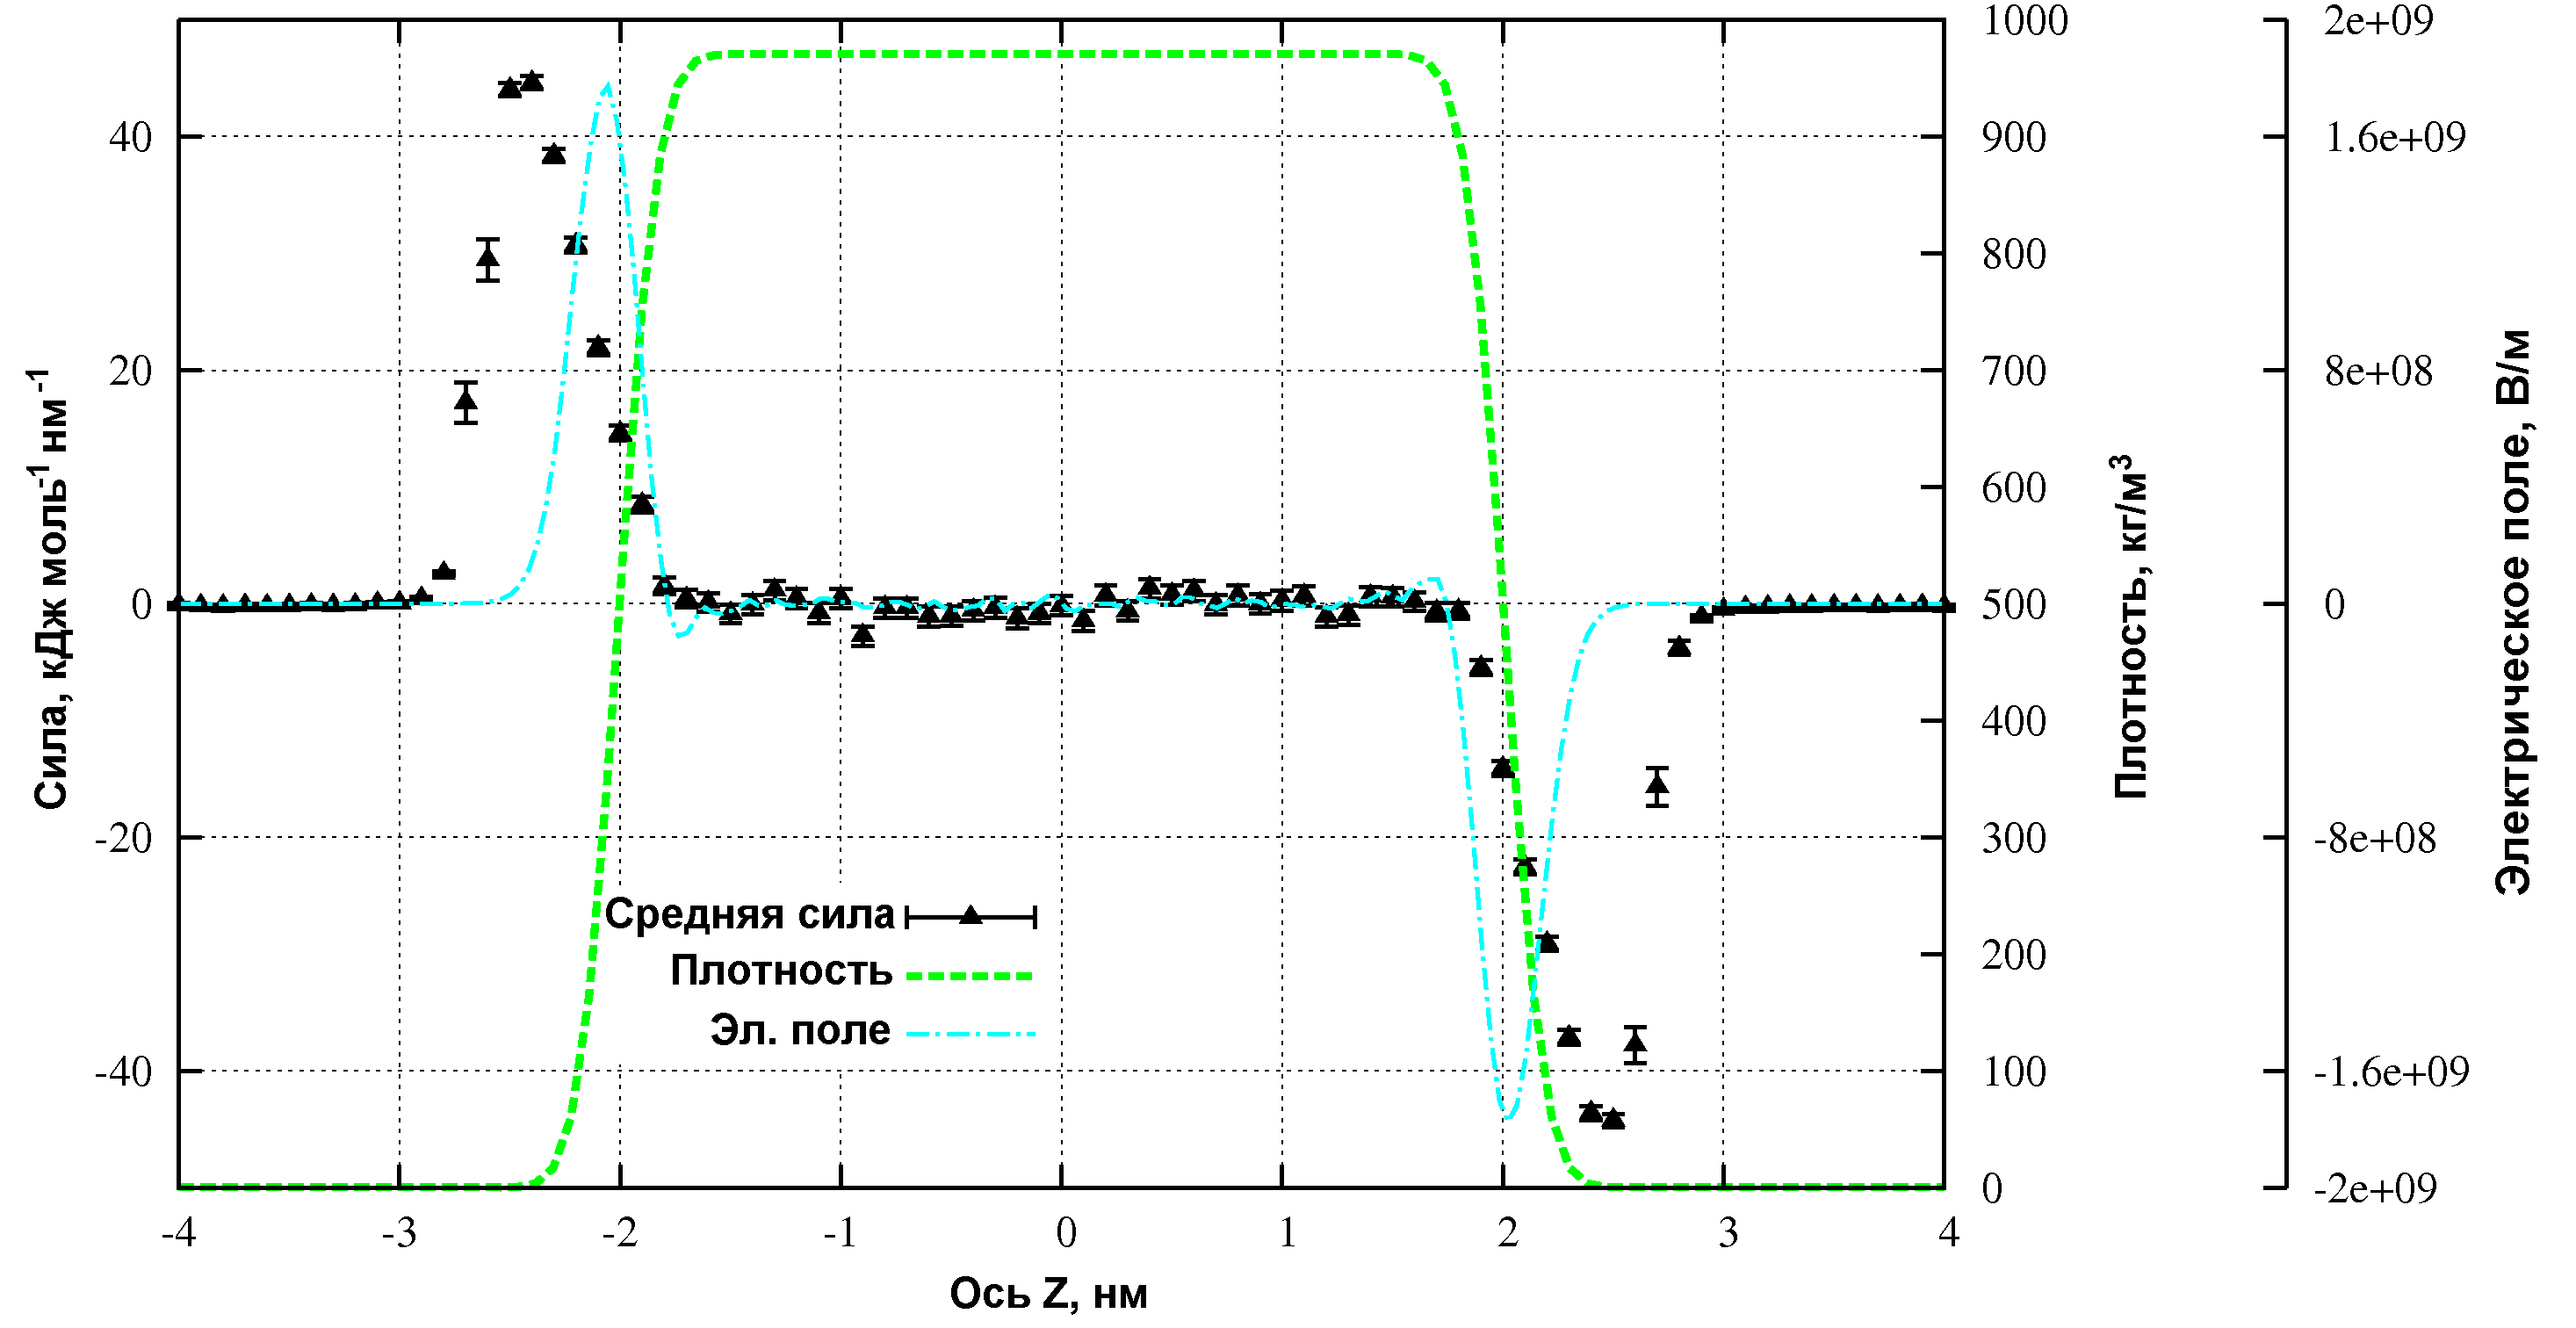
\includegraphics[width=16cm,height=8cm]{mf_d_field}
\caption{\label{mf_d_field}Профиль среднего электрического поля (пунктирно-точечная линия), профиль средней силы для одной молекулы воды (треугольники с погрешностями) как функция Z. Профиль плотности дан для сравнения (пунктирная линия).}
\end{figure}

Чтобы проанализировать ориентационное упорядочение молекул на границе мы построили
средний косинус угла с нормалью и параметр порядка $P_2(\cos{\theta})=<(3\cos{\theta}^2-1)/2>$ как функцию Z (Рис. \ref{orddens}). Видно, что дипольные моменты предпочтительно
ориентированы вдоль границы раздела. Параметр порядка $P_2(\cos{\theta})$  зануляется уже на расстоянии 0.5 нм за поверхностью Гиббса. Также небольшая ориентация диполей по нормали приводит к образованию заряженного бислоя на поверхности и соответствующего среднего электрического поля (Рис. \ref{mf_d_field}), которое достигает значений $1.7*10^{9}$ В/м в узкой области 0.7 нм около поверхности Гиббса.
Поверхностное натяжение было рассчитано на осове диагональных компонент тензора давлений по формуле $\gamma_0=\frac{L_z}{2}(P_{zz}-0.5(P_{xx}+P_{yy}))$. Получена величина $\gamma_0=51.2\pm0.8$ мН/м. Если добавить к этой величине аналитическую поправку возникающую из-за обрезки потенциала Леннард-Джонса, то получится значение 
$\gamma=55.4$ мН/м, это значение занижено по сравнению с экспериментальным (71.6 мН/м при 300K \cite{chem_handbook} ), но находится в хорошем согласии со значениями для модели SPC \cite{smith_surften}. 
 Также на примере молекулы воды была опробована техника расчёта профилей средней силы, на Рис. \ref{mf_d_field} приведён такой профиль. Энергия гидратации молекулы воды, рассчитанная из такого профиля, составляет $-25.5\pm0.7$ кДж/моль.


\subsection{\label{sec:fep_res}Профили свободной энергии}
Основной результат данного исследования -- это набор высокоточных профилей средней силы и свободной энергии для аналогов боковых цепей аминокислот на границе вода/пар. 
Типичные профили средней силы, свободной энергии и концентрации исследуемых молекул представлены на Рис. \ref{4pmf}. Симметричный вид профилей и малые значения статистических погрешностей свидетельствуют о достаточности проведённой выборки. Форма профилей средней силы похожа для всех молекул.

Рассмотрим более детально процесс сольватации с точки зрения полученных профилей.
При расстоянии более 1 нм от поверхности (здесь и далее под положением поверхности понимается положение поверхности Гиббса) нет заметного взаимодействия между молекулой и водным слоем. При дальнейшем приближении к водному слою появляется притягивающая сила, которая, очевидно, обусловлена дисперсионными и электростатическими взаимодействиями. Сила притяжения достигает своего максимума приблизительно на расстоянии 0.5 нм до поверхности Гиббса и далее сходит на нет около границы раздела. Эта область, в которой действует сила притяжения, единственная вносит отрицательный (способствующий гидратации) вклад в энергию гидратации. В таблице \ref{mean_forces} приведены параметры профилей средней силы для всех изученных молекул. Видно, что для молекул содержащих полярные группы (например, THR', ASN', GLN') максимальные значения силы притяжения намного выше, чем для чисто гидрофобных молекул. Приблизительно в районе поверхности Гиббса средняя сила обращается в ноль, что соответствует адсорбционному минимуму на графиках свободной энергии (см. Рис. \ref{4pmf}). Визуальное рассмотрение (Рис. \ref{butane_snapshots}) показывает, что максимум силы притяжения всё ещё соответствует достаточному удалению молекулы от молекул воды, хотя уже заметно некоторое возмущение водного слоя. Когда молекула продвигается далее внутрь водного слоя, возникает выталкивающая сила, которая препятствует дальнейшему погружению молекулы в воду. Причина этой силы, очевидно, может быть приписана проявлению гидрофобного эффекта: молекула вещества нарушает сеть водородных связей молекул воды, что приводит к потере энтропии молекул воды из-за сниженной подвижности последних в округе сольватируемой молекулы. Нужно отметить, что эта сила выталкивания присутствует для  всех веществ (см. Таблицу \ref{mean_forces}), точнее во всех случаях сила выталкивания оказывается сильнее силы притяжения в области сразу за поверхностью Гиббса.
Сила выталкивания пропадает при погружении молекулы на глубину 0.5-0.7 нм в зависимости от размера молекулы. После этого начинается область по своим характеристикам, неотличимая от объёма, где средняя сила взаимодействия равна нулю.
Для некоторых молекул (PHE' ,ILE' ,VAL') есть подозрение, что после области выталкивания существует опять небольшая область притяжения длиной 0.2-0.3 нм, но статистическая достоверность этого утверждения не велика.  Однако присутствие такой области приведёт к возникновению ещё одного максимума на графике свободной энергии, который иногда называют барьером десольватации, который кинетически затрудняет выход растворённого вещества из растворителя и обратно. Тот факт, что средняя сила обращается в ноль уже на расстоянии 0.5-0,7 нм за поверхностью раздела, говорит о том, что на этом расстоянии уже практически отсутствуют поверхностные эффекты влияющие на сольватацию, то есть приблизительно слой толщиной в две молекулы воды экранирует поверхность от молекулы.
\begin{table}[p]

	\begin{tabular}{lcc}
	 & $F^{max}_{at}$,кДж моль$^{-1}$нм$^{-1}$ & $F^{max}_{ex}$,кДж моль$^{-1}$нм$^{-1}$\\
	\hline
ALA'  &  5.0  &  25.8 \\
VAL'  & 10.8  &  33.1\\
LEU'  & 13.0  &  36.2\\
ILE'  & 13.1  &  34.9\\
CYS'  & 19.3  &  21.7\\
MET'  & 25.3  &  28.5\\
SER'  & 41.7  &  12.3\\
THR'  & 44.9  &  18.4\\
TYR'  & 51.3  &  27.2\\
PHE'  & 29.2  &  26.5\\
TRP'  & 51.2  &  26.5\\
ASN'  & 57.6  &  13.0\\
GLN'  & 59.9  &  20.2
\end{tabular}

	\caption{Максимальные значения средней силы притяжения и отталкивания, действующей на изучаемые молекулы по мере из прохождения через водный слой.}
	\label{mean_forces}
	\vspace{3 in}
\end{table}


\begin{figure}
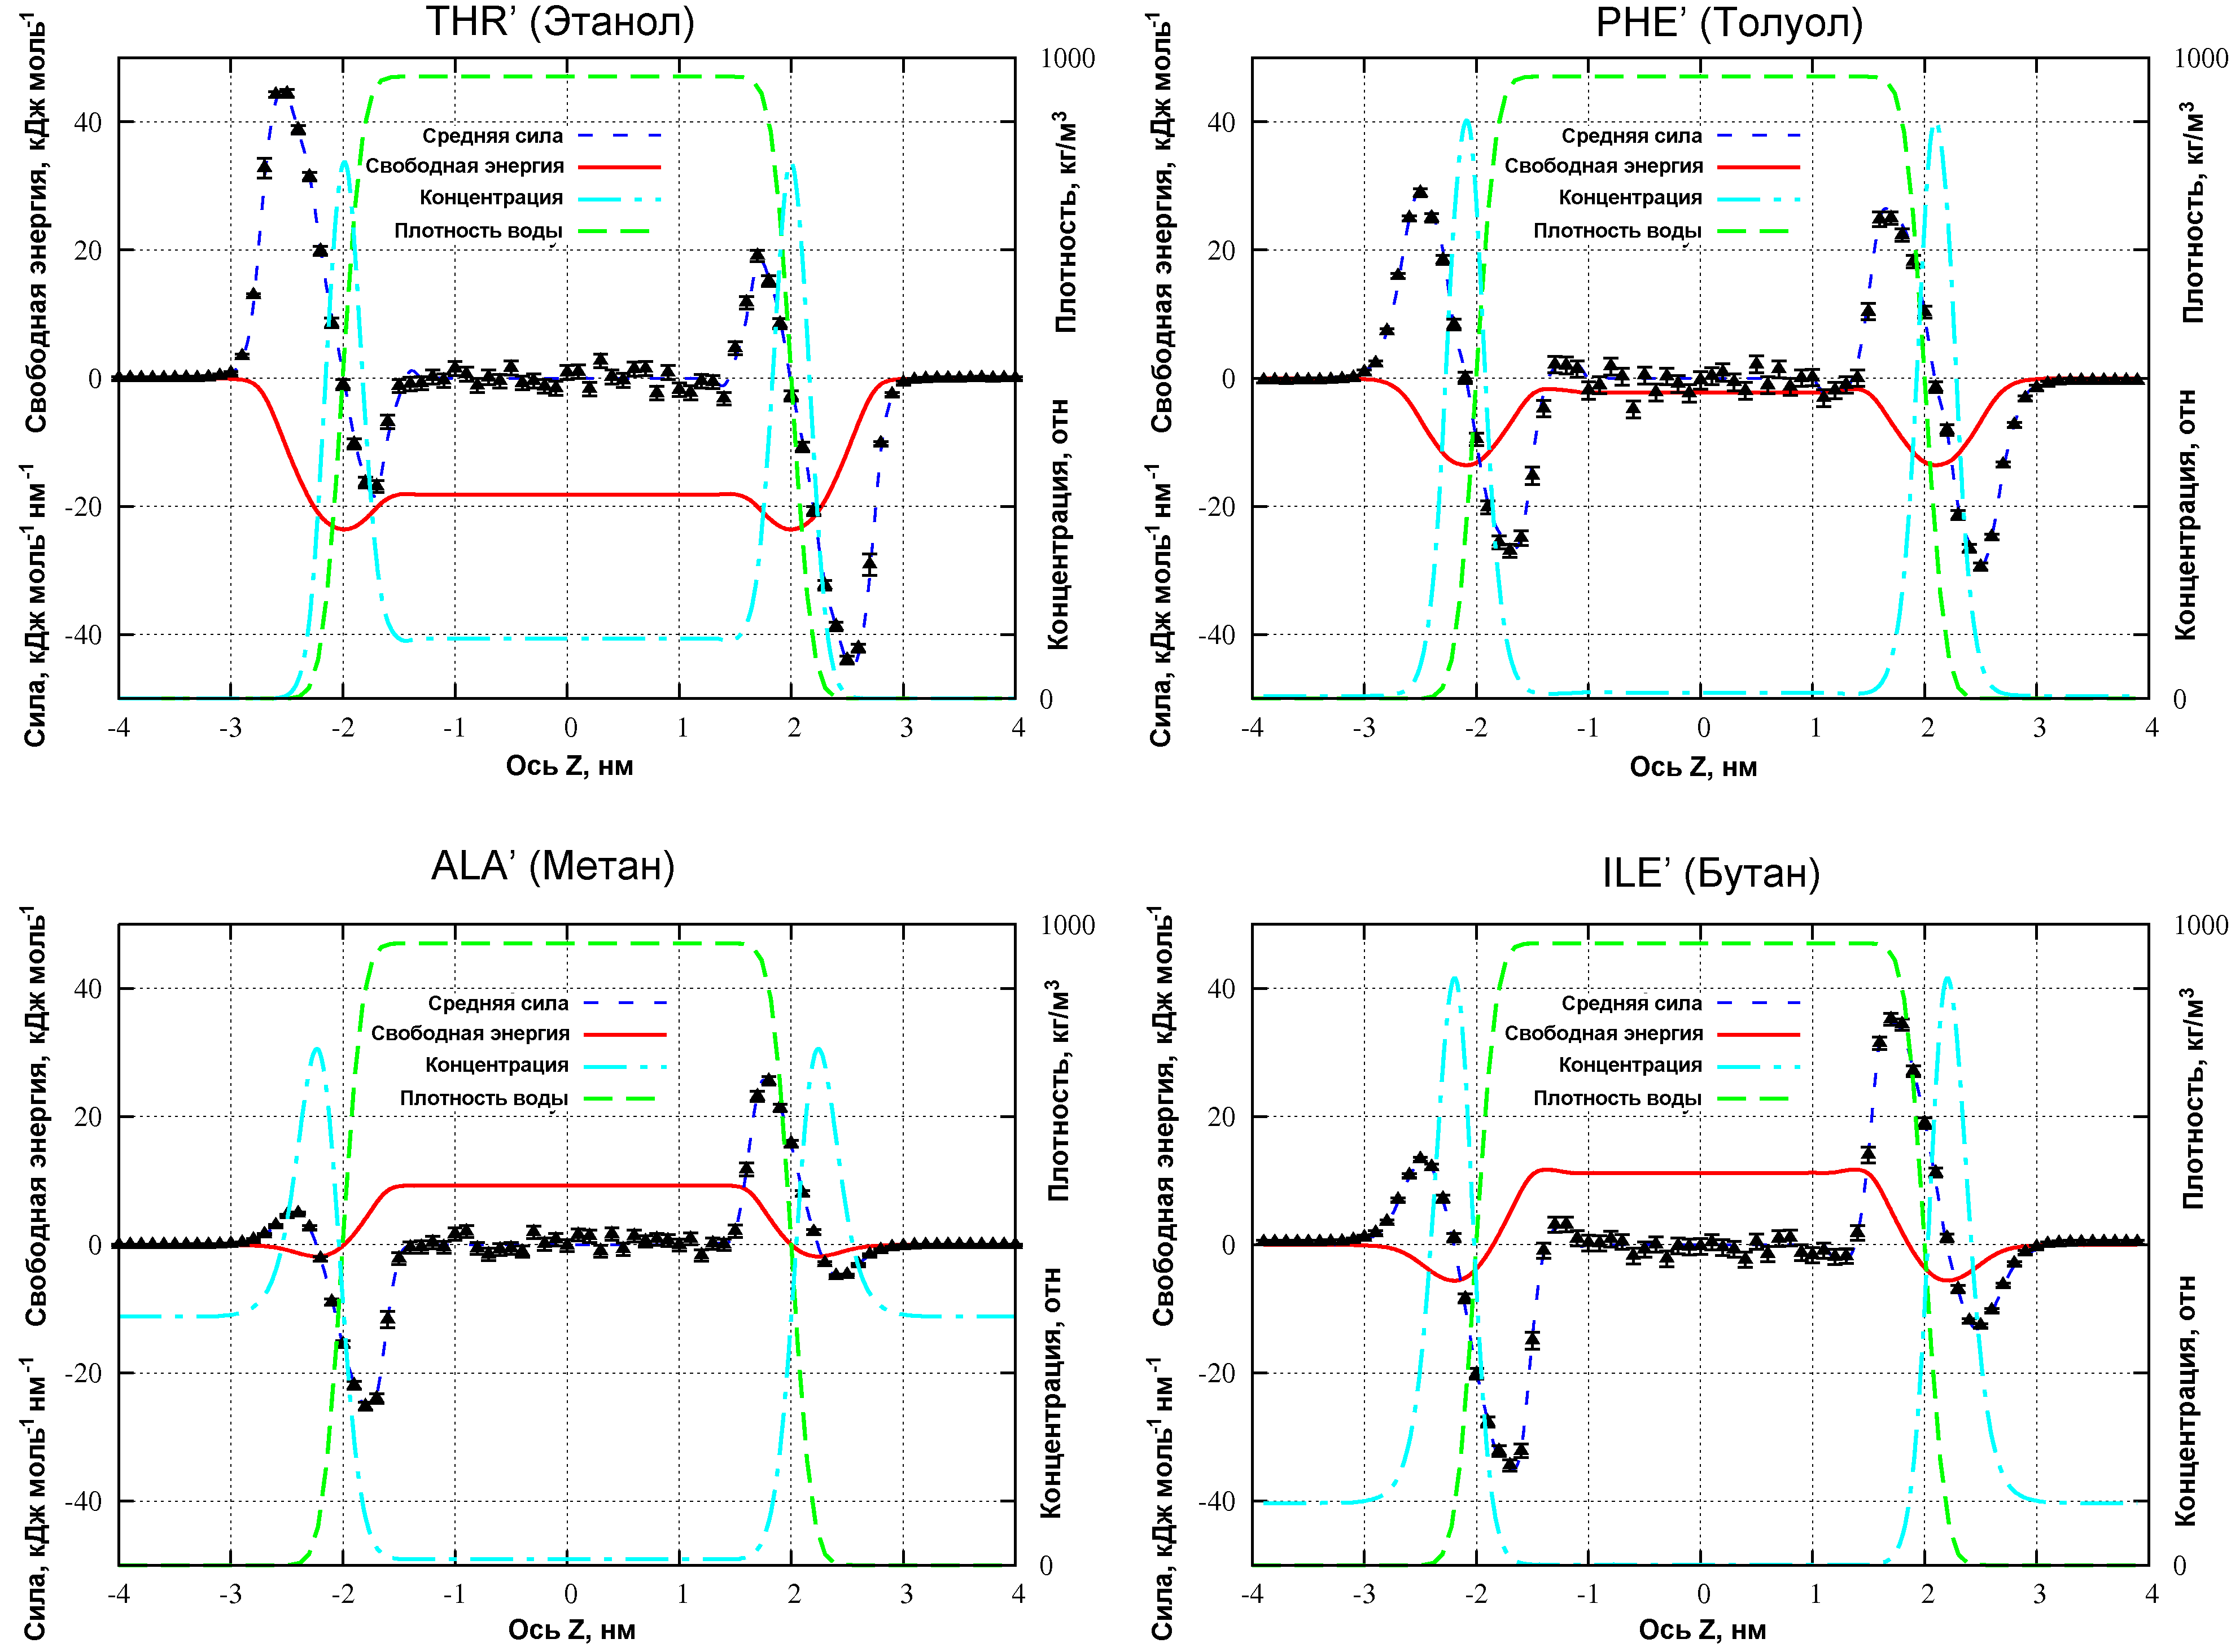
\includegraphics[width=17cm,height=13cm]{4pmf}
\caption{\label{4pmf} Профили свободной энергии для нескольких изученных молекул. Пунктирные линии и точки с отмеченными погрешностями -- профиль средней силы и его сплайн аппроксимация (погрешности отмечены как $\pm$ одно стандартное отклонение). Сплошная линия - профиль свободной энергии, пунктирно-точечная линия - относительный профиль концентрации, рассчитанный по профилю свободной энергии. Для сравнения пунктирной линией отмечен профиль плотности водного слоя.}
\end{figure}

\begin{figure}
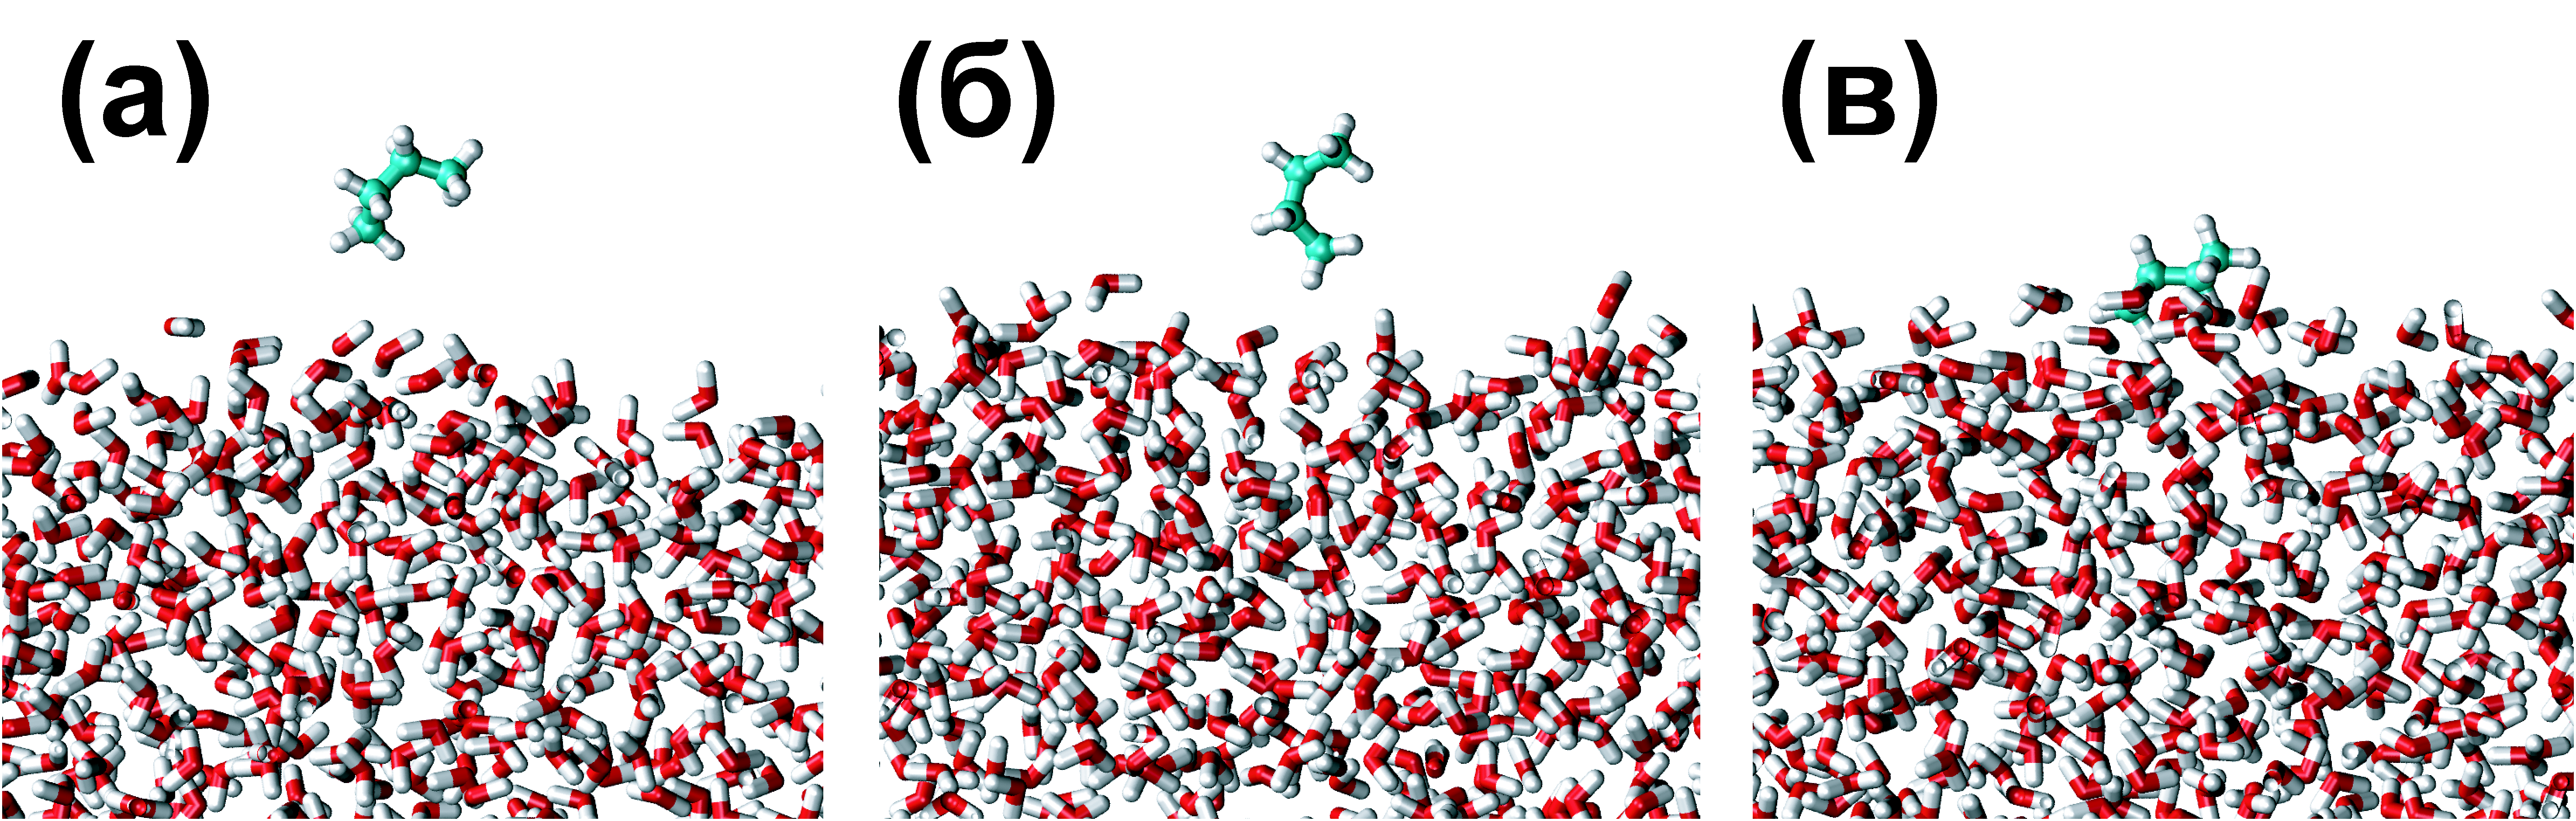
\includegraphics[width=17cm,height=5.5cm]{butane_snapshots}
\caption{\label{butane_snapshots} Мгновенные изображения молекулы бутана во время расчётов на различных расстояниях от границы раздела. Положения соответствующие: (а) максимальной силе притяжения, (b) адсорбционному минимуму, (с) максимальной выталкивающей силе.}
\end{figure}

\subsection{\label{sec:comp_exp}Количественные результаты}
В данном разделе обсудим численные результаты расчётов энергий гидратации и адсорбции. Энергии гидратации были определены двумя способами: как значения профилей свободной энергии в середине слоя, и с помощью метода Беннетта (BAR) из расчётов в объёме. Последние результаты, несомненно, более надёжные, поскольку мало зависят от конечномерных эффектов, дают адекватную оценку статистической погрешности, а также сам метод является методологически хорошо изученным. Поэтому результаты этого метода будут использоваться для критической оценки результатов расчёта профилей свободной энергии.
Результаты обоих методов, а также экспериментальные значения приведены в таблице \ref{hydr_fe}.

\begin{table}[p]
\caption{Энергии гидратации боковых цепей аминокислот, полученные различными методами (методом Беннетта и по профилям свободной энергии), и экспериментальные результаты. Для метода Беннетта статистическая погрешность приведена как одно стандартное отклонение.}
	\label{hydr_fe}

\begin{threeparttable}	
	\begin{tabular}{lccc}
	 & $G^{hydr}_{BAR}$,кДж моль$^{-1}$& $G^{hydr}_{PMF}$,кДж моль$^{-1}$& $G^{hydr}_{exp}$,кДж моль$^{-1}$\tnote{a}\\
	\hline

ALA'  &$  9.20\pm0.04 $& $9.3\pm0.6\tnote{b} $&   8.12  \\
VAL'  &$ 10.1 \pm0.1  $&$ 10.9\pm0.7$ &   8.33  \\
LEU'  &$ 10.57\pm0.08 $&$ 11.3\pm0.8$ &   9.54  \\
ILE'  &$ 10.5\pm 0.3  $&$ 11.7\pm0.7$ &   9.00   \\
CYS'  &$ -2.24\pm0.06 $&$ -1.2\pm0.6$&  -5.19  \\
MET'  &$ -1.74\pm0.18 $&$ -0.5\pm0.7$&  -6.19   \\
SER'  &$-19.2\pm 0.1  $&$ -18.9\pm0.6$& -21.17  \\
THR'  &$-18.65\pm0.13 $&$ -18.1\pm0.7$& -20.42   \\
TYR'  &$-22.33\pm0.18 $&$ -20.5\pm0.9$& -25.56   \\
PHE'  &$ -3.26\pm0.11 $&$ -1.6\pm0.8$&  -3.18  \\
TRP'  &$-18.7\pm 0.3  $&$ -15.9\pm0.9$& -24.60   \\
ASN'  &$-35.69\pm0.10 $&$ -33.6\pm0.9$& -40.50   \\
GLN'  &$-36.45\pm0.16 $&$-32.7\pm0.9$& -39.26  \\
\end{tabular}
\begin{tablenotes}	
	\item[a]{Экспериментальные значения из работы \cite{wolfenden_1988}.}
	\item[b]{Статистические погрешности не включают какие-либо систематические погрешности или погрешности силового поля и методологии.}
\end{tablenotes}
\end{threeparttable}

		
	\vspace{3 in}
\end{table}
Результаты полученные методом BAR находятся в очень хорошем согласии с другими работами \cite{shirts_waterff}. Обсуждения совпадения и отличий данных моделирования и эксперимента может быть найдено в работе \cite{shirts_waterff}: основной вывод состоит в том, что корреляция результатов очень хорошая (в нашем случае коэффициент корреляции равен 0.997), однако абсолютные значения оказываются на 2-4 кДж/моль выше, чем экспериментальные.


Из таблицы \ref{hydr_fe} видно, что статистические погрешности значений рассчитанных из профилей свободной энергии несколько выше (около 1 кДж/моль). Видно, что хотя значения энергий для отдельных веществ (5 из 13) в обоих методах согласуются в пределах статистической погрешности, все значения полученные путём интегрирования профиля средней силы завышены относительно ``настоящих'' модельных значений. Несостыковки ранжируются от 0 для ALA' до 4 кДж/моля для GLN'. Причина этих расхождений, на наш взгляд, кроется в (i) невозможности интегрирования хвоста профиля из-за наличия статистической ошибки в значениях силы, (ii) конечном размере водного слоя и (iii) обрезки потенциала Леннард-Джонса при невозможности применения аналитической поправки (что возможно при расчётах в объёме метдом BAR). Приблизительная оценка теряемой энергии при обрезке потенциала Леннард-Джонса в нашем случае будет варьироваться от 0.4 кДж/моль для ALA' до 3 кДж/моль для TRP'. Применение этих поправок уже сильно бы улучшило совпадения результатов. Однако пока алгоритмы учёта таких поправок для негомогенных систем не развиты.

Мы измерили энергии адсорбции двумя способами: используя подход Гиббса и путём измерения значения профиля энергии в минимуме. В подходе Гиббса сначала рассчитывался относительный профиль концентрации, предполагая концентрацию в газовой фазе равной 1 нм$^{-3}$. Затем рассчитывался избыток Гиббса по формуле \ref{excess} и энергия адсорбции оценивалась по формуле \ref{ads_fe_eq}, предполагая толщину границы раздела равной 1 нм, поскольку это обычно была толщина, на которой варьировался профиль свободной энергии.
Оба набора полученных энергий (см. таблицу \ref{ads_fe}) находятся в отличной корреляции (R=0.9996), хотя заметны некоторые отклонения для веществ с низкой поверхностной активностью, для последних, очевидно, метод имеет значение. Хотя значение энергии в минимуме оказалось хорошей оценкой энергии адсорбции, предположительно метод Гиббса является более универсальным и термодинамически корректным. 

% \begin{equation}
% \Gamma^i=\int_{-\infty}^{z_0}(c^i(z)-c^i_1)dz+\int_{z_0}^{\infty}(c^i(z)-c^i_2)dz
% \label{excess}
% \end{equation}

% \begin{equation}
% G_{ads}=-kT\ln{\frac{\Gamma^S}{c^S\tau}}
% \label{ads_fe_eq}
% \end{equation}


\begin{table}[p]
\caption{Сродство изученных молекул к поверхности, характеризуемое идеальными величинами избытка Гиббса (предполагая концентрацию молекул в фазе пара 1 нм$^{-3}$), энергиями адсорбции Гиббса и глубиной энергии адсорбционного минимума. Последняя колонка представляет энергию адсорбции Гиббса по отношению к фазе максимального сродства.}
	\label{ads_fe}	
	\begin{tabular}{lcccc}
	 & $\Gamma^{excess}$,нм$^{-2}$& $G^{ads}_{Gibbs}$,кДж моль$^{-1}$& $G^{ads}_{min}$,кДж моль$^{-1}$&$G^{ads}_{aff}$,кДж моль$^{-1}$\\
	\hline

ALA'  &$  0.544       $&   1.52 &  -1.82 &  1.52\\
VAL'  &$  2.3         $&  -2.08 &  -4.45 & -2.08\\
LEU'  &$  3.8         $&  -3.33 &  -5.64 & -3.33\\
ILE'  &$  3.7         $&  -3.27 &  -5.59 & -3.27\\
CYS'  &$ 14.0         $&  -6.61 &  -8.76 & -4.37\\
MET'  &$ 57.0         $& -10.1  & -12.35 & -8.36\\
SER'  &$ 2.1*10^3     $& -19.12 & -22.03 &  0.08\\
THR'  &$ 4.7*10^3     $& -21.1  & -23.61 & -2.45\\
TYR'  &$ 65.0*10^3    $& -27.63 & -30.05 & -5.30\\
PHE'  &$ 95.0         $& -11.37 & -13.59 & -8.11\\
TRP'  &$ 22.6*10^3    $& -25.0  & -27.47 & -6.3\\
ASN'  &$0.74*10^6     $& -33.71 & -37.03 &  1.99\\
GLN'  &$2.30*10^6     $& -36.52 & -39.15 & -0.02\\
\end{tabular}
	
	
	\vspace{3 in}
\end{table}


Значения энергии адсорбции Гиббса в таблице \ref{ads_fe} представлены относительно фазы максимального сродства (как обычно делается в экспериментальных работах). Можно сказать, что все вещества являются поверхностно активными в том плане, что в профилях свободной энергии у них есть адсорбционный минимум. Однако конченые значения энергии адсорбции всегда являются относительными поскольку зависят от определения стандартных состояний и условной толщины границы раздела.

К сожалению, в литературе встречается мало экспериментальных данных, с которыми можно было бы сравнить полученные численные данные. Бул и Бриз \cite{bull_breese} ввели шкалу энергий адсорбции для боковых цепей аминокислот, руководствуясь данными по измерению поверхностного натяжения для цвиттерионых аминокислот и применяя предположение об аддитивности вкладов различных молекулярных групп. Однако, если предположение об аддитивности достаточно хорошо себя зарекомендовало при оценках энергий сольватации, то в случае измерения энергий адсорбции справедливость такого предположения вызывает сомнения.
Коэффициент корреляции шкалы Була и Бриза с модельными результатами по адсорбции составляет 0.65.

Измерения избытка Гиббса для метанола и этанола были проведены с помощью нейтронного рассеяния \cite{eth-excess-exp,meth-excess-exp} и равны  2.5*10$^{-10}$ моль*см$^{-2}$ и (3-5)*10$^{-10}$ моль*см$^{-2}$, соответственно, при объёмной концентрации в 0.0012 моль*см$^{-3}$. Эти данные находятся в разумном согласии с результатами нашей модели равными 1.2*10$^{-10}$ моль*см$^{-2}$ и 2.6*10$^{-10}$ моль*см$^{-2}$ для этого случая. По данным работы \cite{atmgas_excess-exp} на основании измерения поверхностного натяжения энергия адсорбции метанола из газовой фазы составляет $-15.2\pm0.5$ кДж/моль, в то время как из наших расчётов следует величина -19.2. кДж/моль.


Следуя идеям статьи Охапкина и др. \cite{okhapkin_amino}, нами были построены двумерные диаграммы сродства молекул к объёмной и поверхностной фазе воды (Рис. \ref{diagr}) по двум параметрам: энергии гидратации и энергии адсорбции относительно фазы максимального сродства. Видно, что изученные молекулы покрывает достаточно большую область энергий адсорбции и гидратации. Некоторые молекулы обладают сходными характеристиками, например, (i) PHE' и MET', (ii) VAL',ILE' и LEU',  (iii) ASN' и GLN'. Однако, в общем можно заключить, что корреляции между энергиями адсорбции относительно фазы максимального сродства и гидратации в нашем случае не наблюдается, эти характеристики являются независимыми и в то же время достаточно простыми параметрами, описывающими взаимодействие растворителя с другими веществами, которые могут использоваться для улучшения и уточнения молекулярных моделей и силовых полей подобно тому, как для этого используются только энергии гидратации \cite{gromos_hydr}.

\begin{figure}
\centering
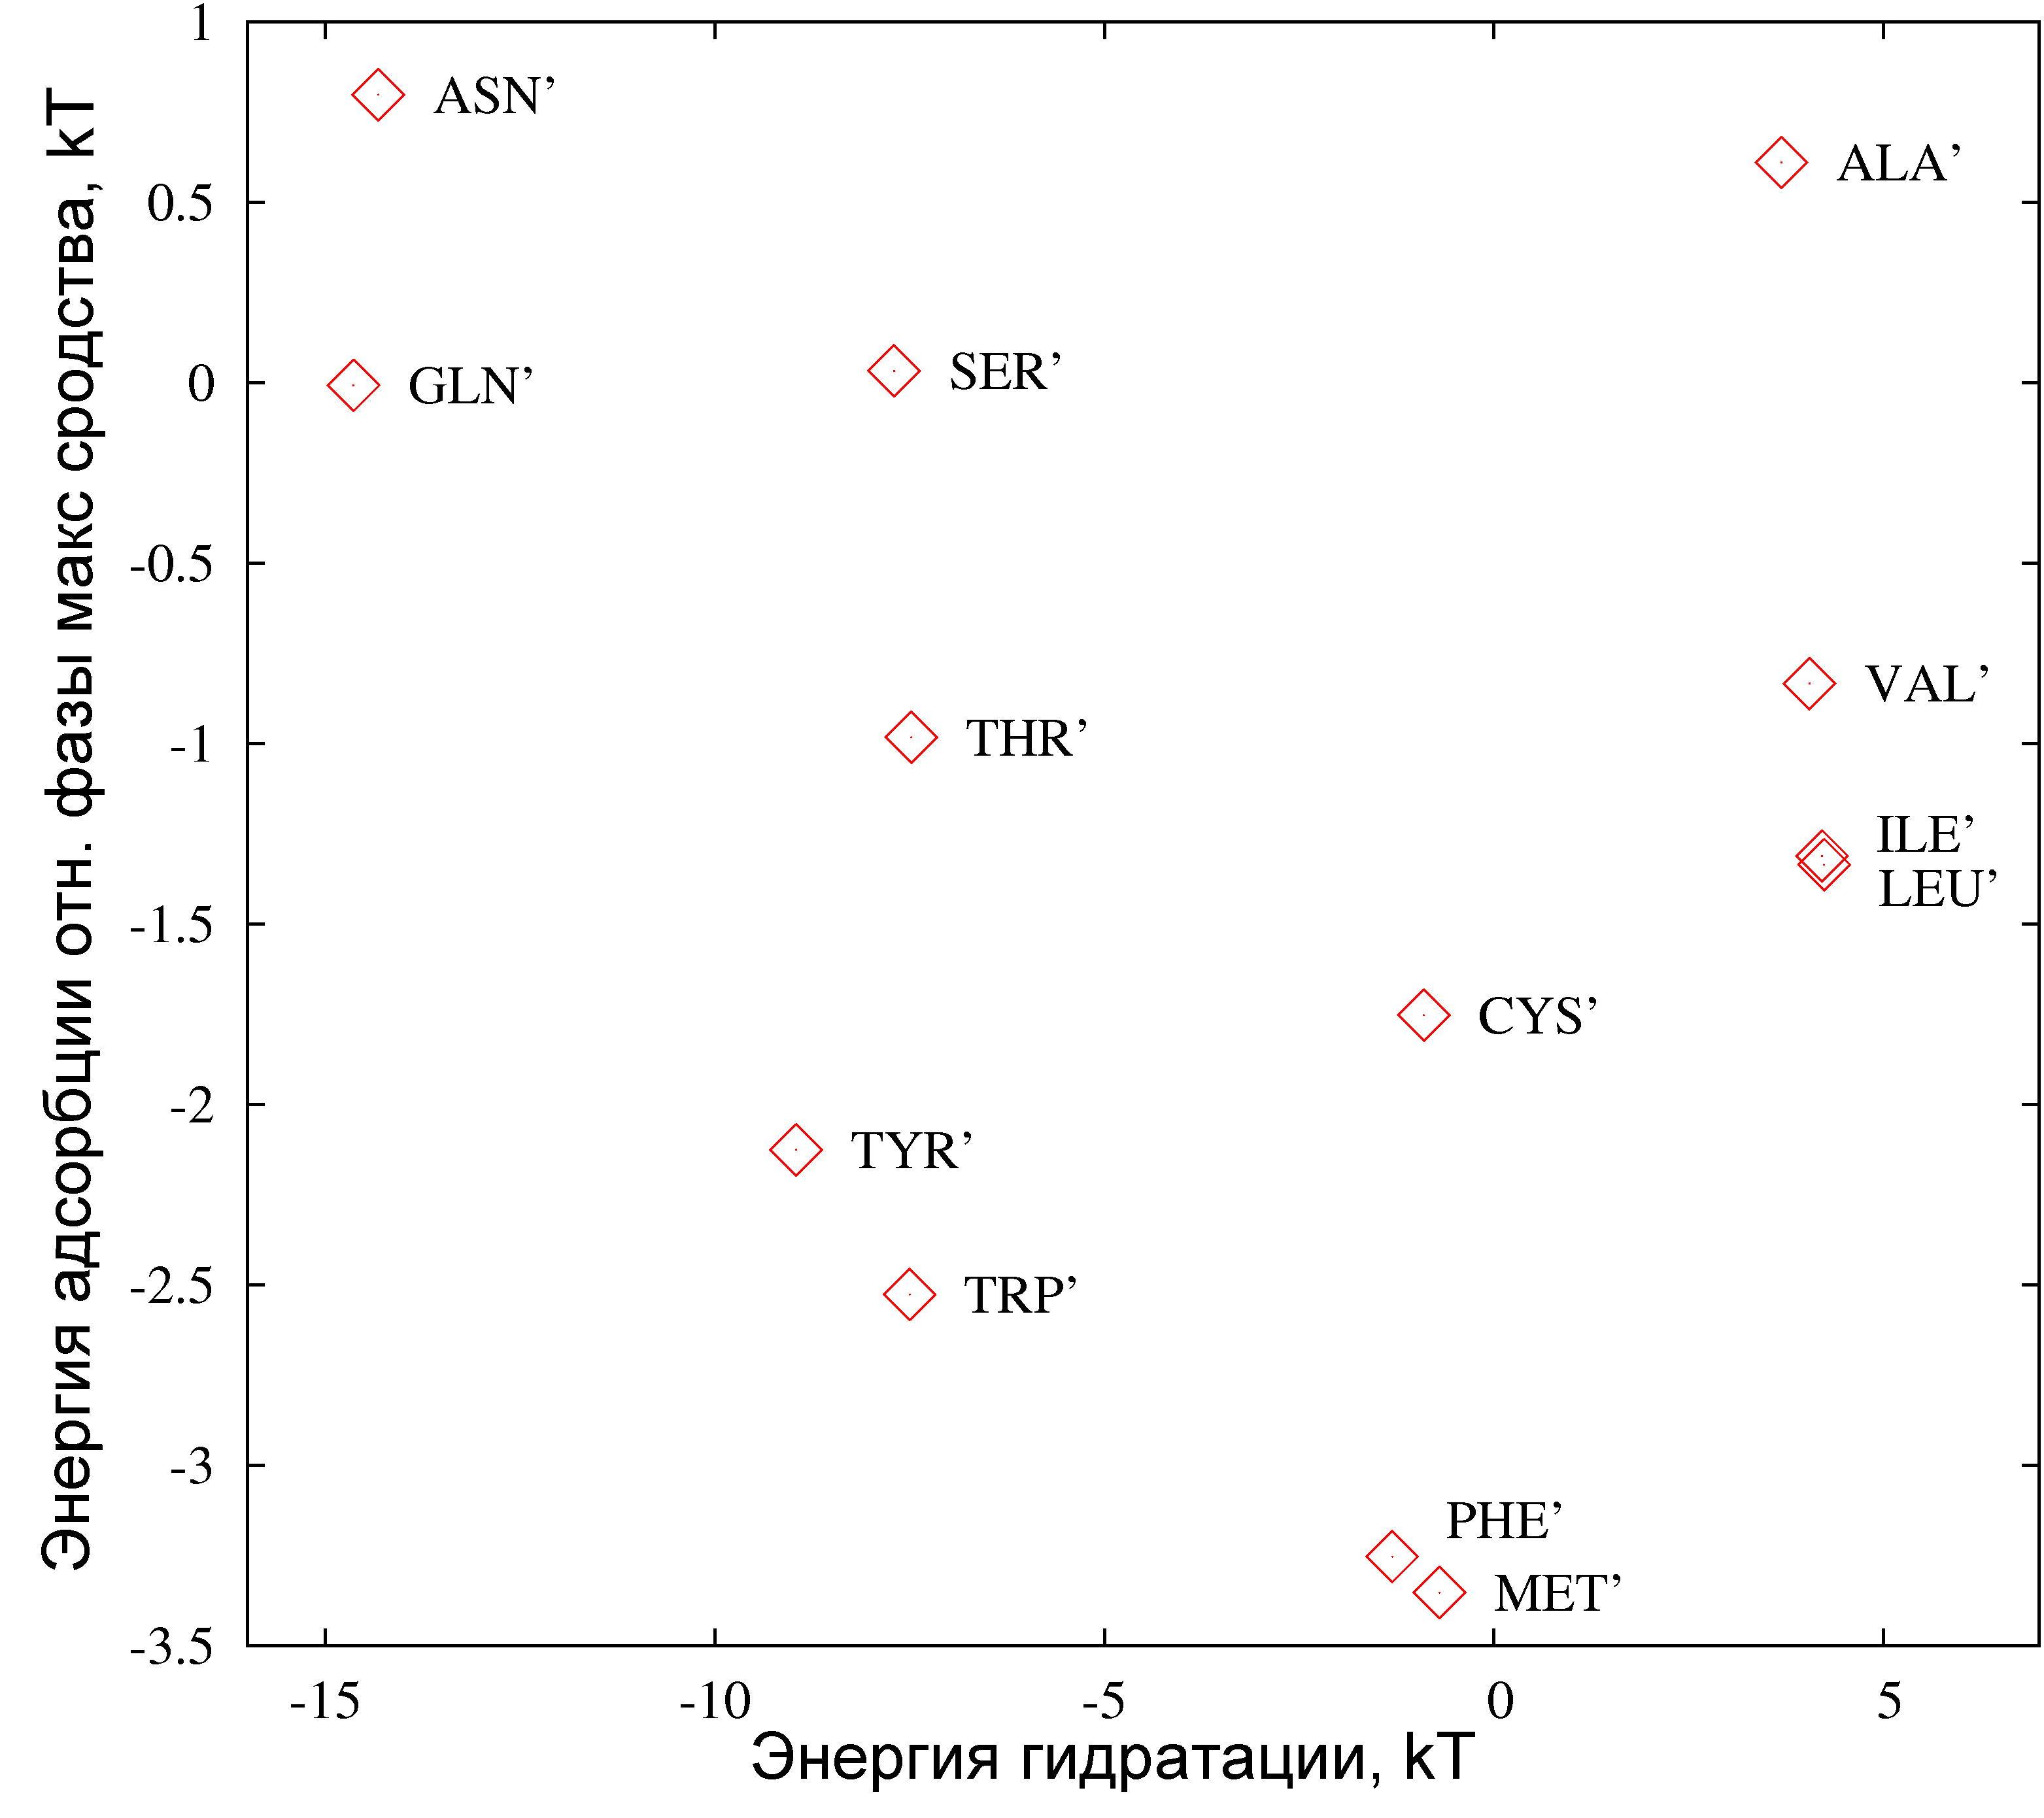
\includegraphics[width=10cm]{diagr}
\caption{\label{diagr} Двумерная классификационная диаграмма для исследованных веществ в координатах энергия гидратации - энергия адсорбции относительно фазы максимального сродства.}
\end{figure}

\begin{figure}
\centering
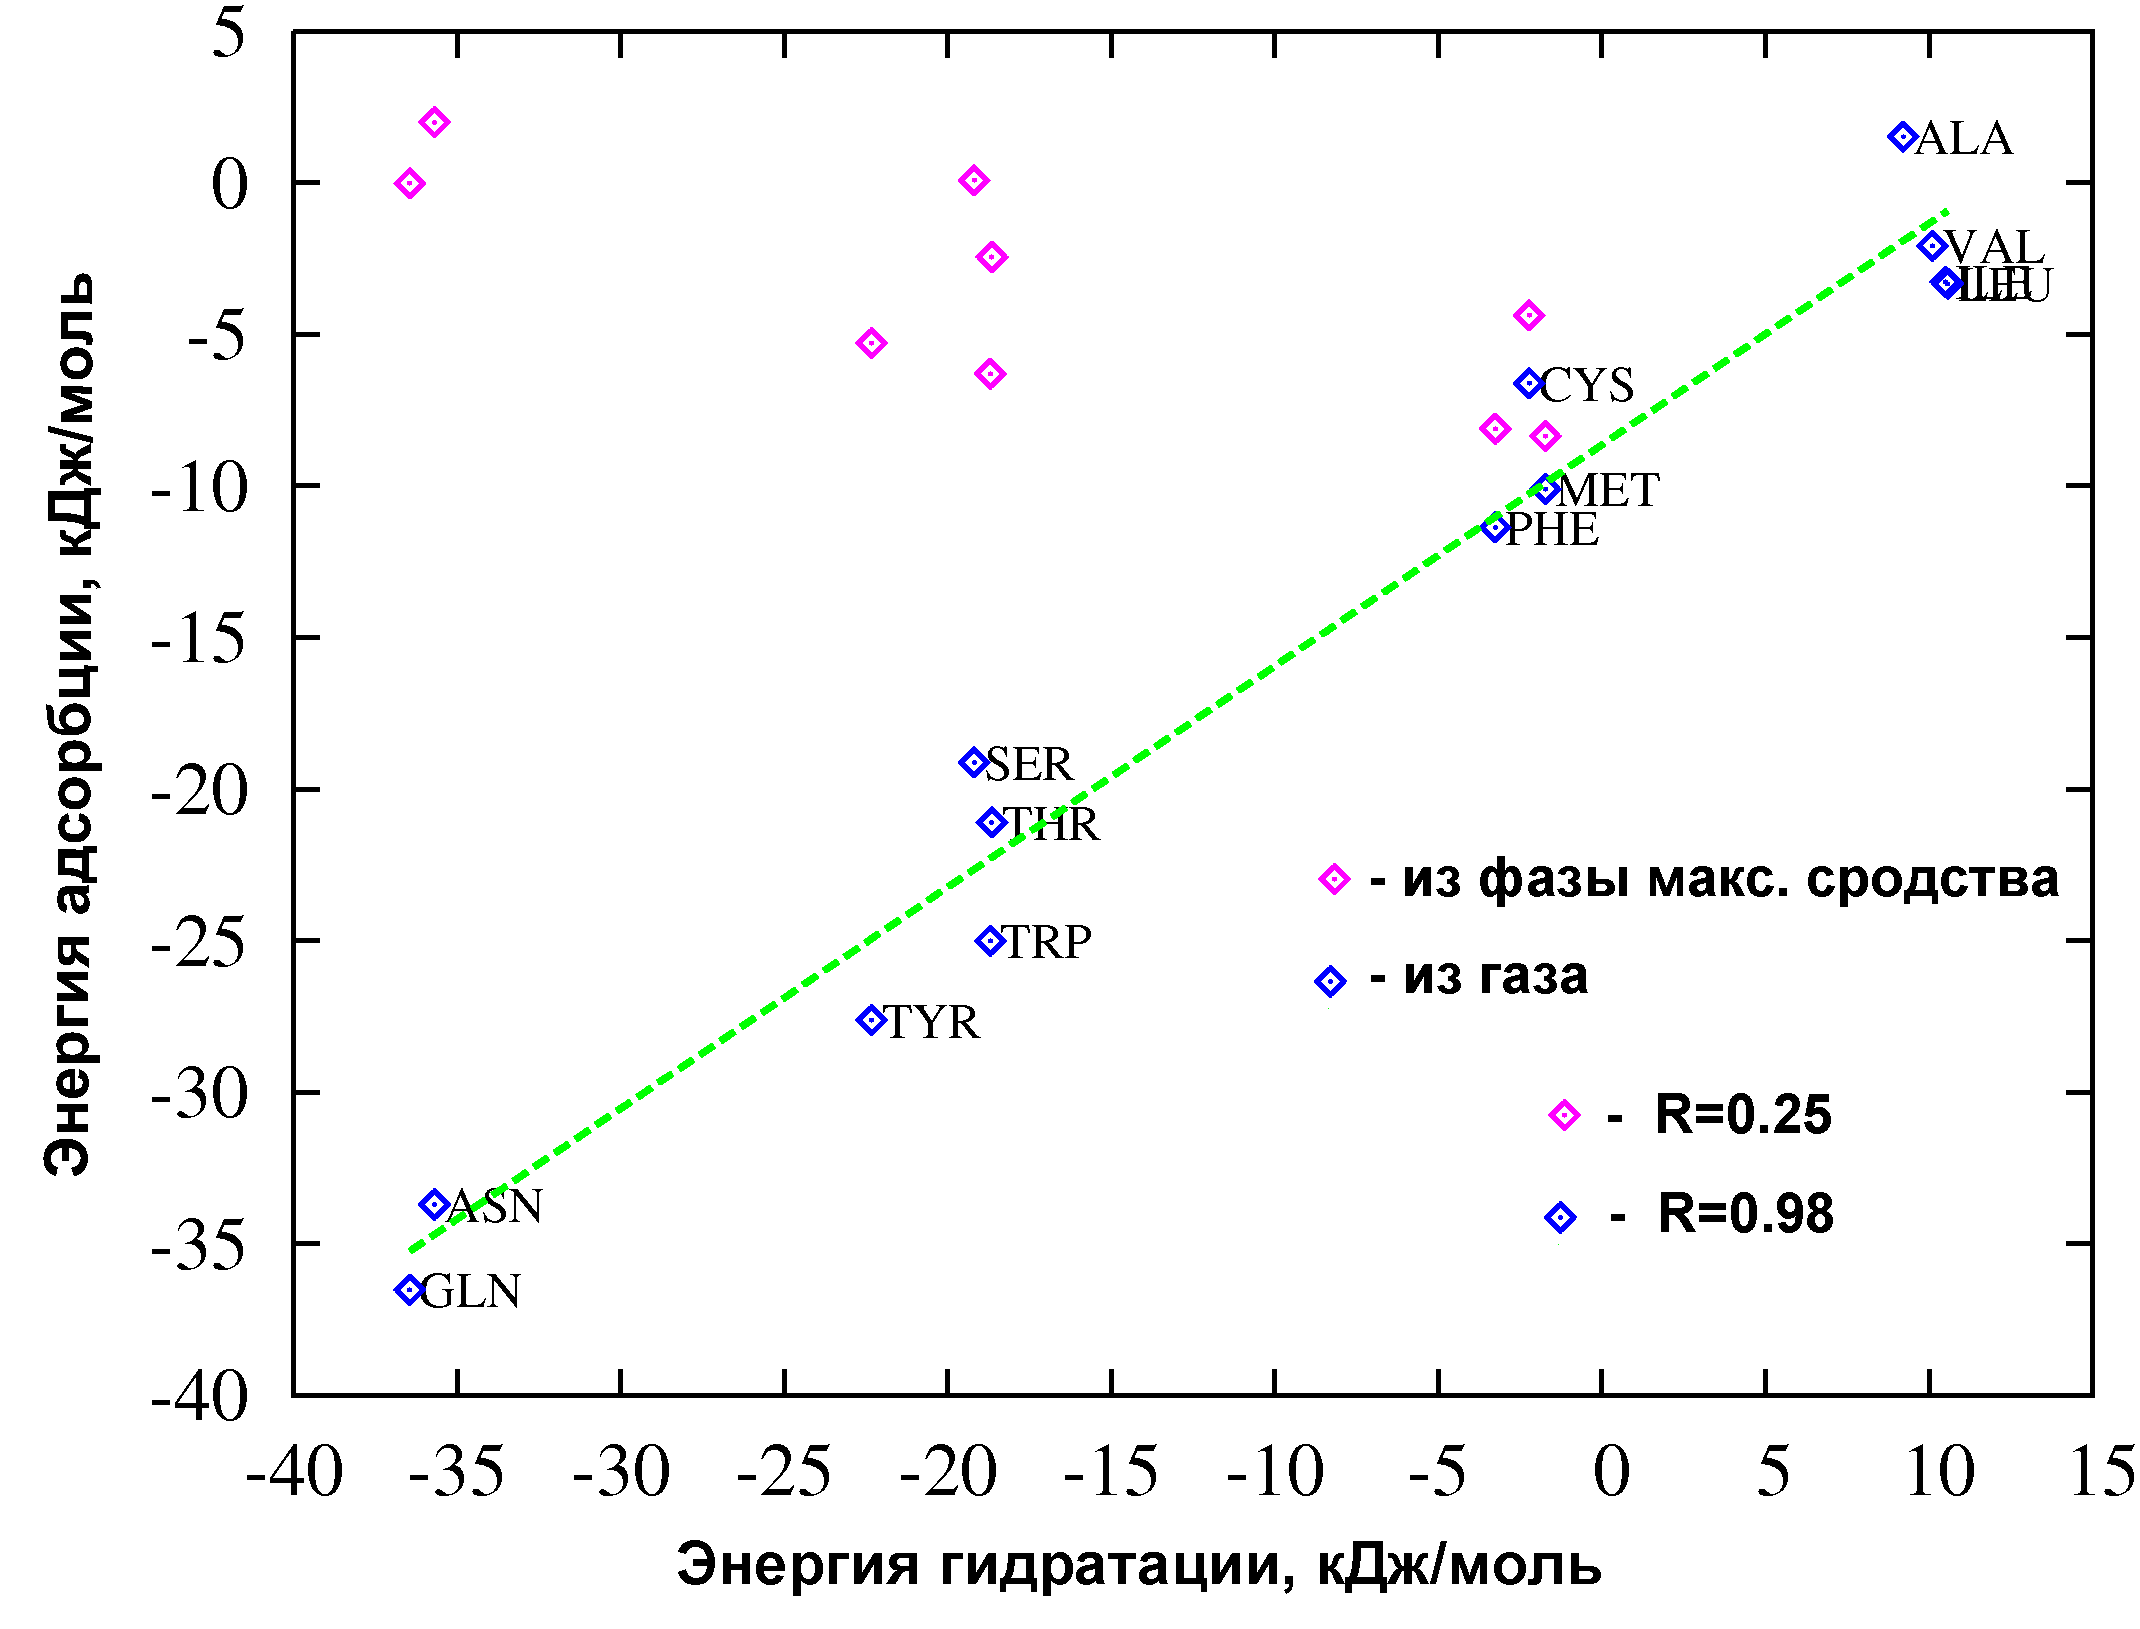
\includegraphics[width=10cm]{cor_ads_hydr_affin}
\caption{\label{cor_ads_hydr_affin} График корреляций между энергиями гидратации и адсорбции.}
\end{figure}


\subsection{\label{sec:comp_correl}Корреляционный анализ }
Поскольку на данный момент не существует систематических данных по экспериментальному измерению энергий адсорбции, изученных боковых цепей аминокислот, то представляется интересным провести анализ корреляций между полученными данными и статистическими шкалами предложенными в главе 4. Соответствующие коэффициенты корреляции, а также коэффициенты корреляции статистических шкал с экспериментальными, рассчитанные только для 13 исследованных соединений, представлены в таблице \ref{tab:comp_corr}. Как видно из таблицы, по коэффициентам корреляции шкала $G_{Gibbs}^{ads}$ достаточно хорошо совпадает со шкалой гидратации ($V>W$). Это вызвано тем, что для полярных гидрофильных молекул энергия адсорбции (глубина адсорбционного минимума) не сильно отличается от энергии гидратации. Для неполярных молекул такое утверждение не справедливо, энергия гидратации там плохо коррелирует с энергией адсорбции, однако, величины этих энергий не велики и коэффициент корреляции они портят не сильно. Демонстрация этого факта приведена на рис. \ref{cor_ads_hydr_affin}.

%\begin{turnpage}
\begin{table}
\caption{\label{tab:comp_corr} Коэффициенты корреляции энергий адсорбции ($G_{Gibbs}^{ads}$), полученных в результате численного моделирования и экспериментальных шкал  со статистическими данными, полученными в главе 4. Корреляции рассчитывались только для 13 незаряженных аминокислот.}

	\begin{tabular}{l|ccc|cc}
	        & ``10-20'' & ``50-60'' & ``95-105''& $G_{Gibbs}^{ads}$ & $G_{affin}^{ads}$\\
	   \hline
$G_{Gibbs}^{ads}$ & 0.48  &  0.88  & 0.7 & 1 & 0.17\\
$G_{affin}^{ads}$&     0.2         &  0.53         &  0.7     & 0.17  & 1\\
V>W&0.46&0.87&0.73 & 0.98 & 0.23 \\
CH>W&0.19&0.91&0.92 & 0.81 & 0.56\\
O>W&0.09&0.76&0.88 & 0.48 & 0.77\\


\end{tabular}

	
\end{table}
%\end{turnpage}
	 

\section{Выводы главы \ref{part3_free_energy}}

\textbf{Значимость и актуальность}\\
Рост возможностей современных компьютерных систем постепенно позволяет переходить на качественно новый уровень в моделировании молекулярных процессов: вычисления свободных энергий, энтропий и других термодинамических характеристик реальных молекулярных систем на основе их атомистических моделей с приемлемой точностью. Основные трудности таких вычислений связаны с (i) необходимостью осуществления обширной выборки состояний системы в различных статистически значимых конформациях, число которых быстро возрастает с увеличением сложности энергетического ландшафта системы, (ii) необходимостью понимания применимости существующих силовых полей, параметризованных по различным ``энергетическим'' характеристикам молекул, для вычислений такого рода, 
(iii) умением соотносить характеристики рассчитанные в системах небольшого размера с настоящими термодинамическими характеристиками и необходимостью разрабатывать соответствующие методы.
Особый интерес такие методы вызывают в связи с моделированием и построением моделей различных биологических структур (в частности белков), в самоорганизации которых важную роль играют гидрофобные взаимодействия, как раз носящие энтропийный, сильно статистический характер и, без адекватного описания которых на молекулярном уровне,
рассмотрение задач о самосборке и стабильности таких структур в компьютерном моделировании весьма сложно. Заметим, что выигрыш в свободной энергии при сворачивании белков весьма небольшой (10-20 ккал/моль), что накладывает дополнительные требования к качеству воспроизведения взаимодействий в моделировании. Короме того, поскольку биологические системы являются зачастую микрогетерогенными, (например, растворитель и ядро белка, актуальным является также корректное воспроизведение взаимодействий для отдельных молекул как в объёме фазы, так и на поверхности, что в свою очередь влияет на такую характеристику как поверхностное натяжение.
В данной работе освещён один из фундаментальных и одновременно методологических аспектов компьютерного моделирования белково-подобных систем, рассмотрено взаимодействие различных типов аминокислот с границей раздела фаз вода/воздух. Результаты работы с одной стороны дают фундаментальную информацию о взаимодействии аминокислот с поверхностью воды, с другой стороны предоставляют численные результаты для оценки точности широкоиспользуемых в настоящее время силовых полей и их совершенствования.

\textbf{Проведённые работы}\\
Была разработана методика моделирования, исследована структура (в том числе ориентационная) и характеристики водного слоя толщиной 4 нм. Разработана методика и вычислены профили свободной энергии для боковых цепей аминокислот вдоль нормали к границе водного слоя. Обсуждается вопрос о методах расчёта энергии адсорбции, предложено два метода и проведены оценки энергии адсорбции для боковых цепей аминокислот. Независимым способом путём ``выключения'' взаимодействия между молекулой и растворителем в объёме проведена оценка свободной энергии гидратации исследуемых молекул, проведено сравнение энергий получаемых двумя способами. На основании расчётов проведена оценка корреляций между энергиями гидратации и адсорбции (как абсолютных, так и относительно фазы максимального сродства), также проведена оценка корреляций шкал с результатами статистического анализа главы 4. 

\textbf{Положение работы в контексте аналогичных работ и новизна}\\
Расчёты свободных энергий гидратации для боковых цепей аминокислот были проведены целым рядом исследователей для различных силовых полей. В нескольких работах авторы очень внимательно относились к возможной зависимости параметров моделирования на получаемые результаты и получали результаты с достоверной оценкой погрешностей. Следует отметить, что данная тема является достаточно широко исследуемой в связи с вышеозвученными аргументами. Расчёт профилей свободной энергии для небольших молекул (в основном газов) на границе с водой проводился некоторыми исследователями, однако, на взгляд автора, в имеющихся работах выполнен достаточно небрежно. Что же касается систематического расчёта профилей свободной энергии для боковых цепей аминокислот на границе с водой, то таких работ найдено не было, поэтому можно утверждать, что данная работа выполнена впервые. Предложенный автором способ расчёта энергий адсорбции на основе профилей свободной энергии в купе с методом молекулярного моделирования также обладает новизной.




По результатам работы можно сделать следующие выводы, обладающие научной новизной:
\begin{itemize}
\item Профили средней силы для боковых цепей аминокислот на границе вода-воздух приблизительно одинаковы по форме: имеют область притяжения перед поверхностью Гиббса со стороны воздуха, и достаточно узкую (0.6-0.7 нм) область выталкивания за поверхностью Гиббса.
\item Вывод об одинаковой форме профилей средней силы на границе вода/воздух, по-видимому, можно обобщить на весть класс небольших незаряженных молекул.
\item В использованной модели, видимые поверхностные эффекты сольватации для боковых цепей аминокислот исчезают, когда центр масс молекулы погружён на 0.6-0.7 нм в воду по отношению к поверхности Гиббса, что может считаться эффективной глубиной границы раздела для маленьких молекул.
\item Профили свободной энергии для всех молекул обладают минимумом в районе границы раздела, который является результатом баланса между силами притяжения, доминирующими со стороны воздуха, и силами отталкивания, доминирующими со стороны воды, и имеющими энтропийную природу.
\item Глубина минимума свободной энергии находится в хорошей корреляции с энергией адсорбции, рассчитанной по методу Гиббса.
\item С высокой точностью вычислены энергии гидратации и адсорбции для 13 незаряженных веществ-аналогов боковых цепей аминокислот.
\item Показано, что энергия адсорбции из газовой фазы для выбранного набора боковых цепей аминокислот находиться в хорошей корреляции с энергией гидратации.
\item Энергия адсорбции относительно фазы максимального сродства не коррелирует с энергией гидратации и может использоваться как независимая термодинамическая характеристика молекул вещества.
\item Полученные данные для нескольких молекул согласуются с экспериментальными данными и могут применяться для совершенствования силовых полей, однако достоверных систематических данных по оценки энергии адсорбции для всей группы веществ на границе вода-воздух пока в литературе не обнаружено.
\end{itemize}


\subsection{Положения выносимые на защиту}
%положения выносимые на защиту
\begin{enumerate}
  \item Разработаны подходы позволяющие вычислять термодинамические параметры взаимодействия малых органических молекул с водой и ее поверхностью (свободную энергию гидратации и адсорбции) на основе их атомистических моделей.
  \item Систематическое завышение свободной энергии гидратации боковых цепей аминокислот современными силовыми полями (на 0.5 - 2 kT на аминокислоту) является одним из факторов гиперстабильности молекулярно-динамических моделей белков, свидетельствует о необходимости улучшения силовых полей биомакромолекул и молекул воды для моделирования фолдинга белков. 
\end{enumerate}